% A LaTeX template for MSc Thesis submissions to 
% Politecnico di Milano (PoliMi) - School of Industrial and Information Engineering
%
% S. Bonetti, A. Gruttadauria, G. Mescolini, A. Zingaro
% e-mail: template-tesi-ingind@polimi.it
%
% Last Revision: October 2021
%
% Copyright 2021 Politecnico di Milano, Italy. NC-BY

\documentclass{Configuration_Files/PoliMi3i_thesis}

%------------------------------------------------------------------------------
%	REQUIRED PACKAGES AND  CONFIGURATIONS
%------------------------------------------------------------------------------

% CONFIGURATIONS
\usepackage{listings}
\usepackage[dvipsnames]{xcolor} 
\usepackage{parskip} % For paragraph layout
\usepackage{setspace} % For using single or double spacing
\usepackage{emptypage} % To insert empty pages
\usepackage{multicol} % To write in multiple columns (executive summary)
\setlength\columnsep{15pt} % Column separation in executive summary
\setlength\parindent{0pt} % Indentation
\raggedbottom  

% PACKAGES FOR TITLES
\usepackage{titlesec}
% \titlespacing{\section}{left spacing}{before spacing}{after spacing}
\titlespacing{\section}{0pt}{3.3ex}{2ex}
\titlespacing{\subsection}{0pt}{3.3ex}{1.65ex}
\titlespacing{\subsubsection}{0pt}{3.3ex}{1ex}
\usepackage{color}

% PACKAGES FOR LANGUAGE AND FONT
\usepackage[english]{babel} % The document is in English  
\usepackage[utf8]{inputenc} % UTF8 encoding
\usepackage[T1]{fontenc} % Font encoding
\usepackage[11pt]{moresize} % Big fonts


% PACKAGES FOR IMAGES
\usepackage{graphicx}
\usepackage{transparent} % Enables transparent images
\usepackage{eso-pic} % For the background picture on the title page
\usepackage{subfig} % Numbered and caption subfigures using \subfloat.
\usepackage{tikz} % A package for high-quality hand-made figures.
\usetikzlibrary{}
\graphicspath{{./Images/}} % Directory of the images
\usepackage{caption} % Coloured captions
% Coloured captions
\usepackage{amsthm,thmtools,xcolor} % Coloured "Theorem"
\usepackage{float}

% STANDARD MATH PACKAGES
\usepackage{amsmath}
\usepackage{amsthm}
\usepackage{amssymb}
\usepackage{amsfonts}
\usepackage{bm}
\usepackage[overload]{empheq} % For braced-style systems of equations.
\usepackage{fix-cm} % To override original LaTeX restrictions on sizes

% PACKAGES FOR TABLES
\usepackage{tabularx}
\usepackage{longtable} % Tables that can span several pages
\usepackage{colortbl}

% PACKAGES FOR ALGORITHMS (PSEUDO-CODE)
\usepackage{algorithm}
\usepackage{algorithmic}
\usepackage{minted}

% PACKAGES FOR REFERENCES & BIBLIOGRAPHY
\usepackage[colorlinks=true,linkcolor=black,anchorcolor=black,citecolor=black,filecolor=black,menucolor=black,runcolor=black,urlcolor=black]{hyperref} % Adds clickable links at references
\usepackage{cleveref}
\usepackage[square, numbers, sort&compress]{natbib} % Square brackets, citing references with numbers, citations sorted by appearance in the text and compressed
\bibliographystyle{abbrvnat} % You may use a different style adapted to your field

% OTHER PACKAGES
\usepackage{pdfpages} % To include a pdf file
\usepackage{afterpage}
\usepackage{lipsum} % DUMMY PACKAGE
\usepackage{fancyhdr} % For the headers
\fancyhf{}

   %May be necessary if you want to color links
\lstdefinestyle{mystyle}{
    backgroundcolor=\color{lightgray},
    commentstyle=\color{Goldenrod},
    keywordstyle=\color{ForestGreen},
    numberstyle=\tiny\color{RawSienna},
    stringstyle=\color{JungleGreen},
    basicstyle=\ttfamily\footnotesize,
    breakatwhitespace=false,         
    breaklines=true,                 
    captionpos=b,                    
    keepspaces=true,                 
    numbers=left,                    
    numbersep=5pt,                  
    showspaces=false,                
    showstringspaces=false,
    showtabs=false,                  
    tabsize=2
}

\lstset{style=mystyle}
% Input of configuration file. Do not change config.tex file unless you really know what you are doing. 
% Define blue color typical of polimi
\definecolor{bluepoli}{cmyk}{0.4,0.1,0,0.4}

% Custom theorem environments
\declaretheoremstyle[
  headfont=\color{bluepoli}\normalfont\bfseries,
  bodyfont=\color{black}\normalfont\itshape,
]{colored}

% Set-up caption colors
\captionsetup[figure]{labelfont={color=bluepoli}} % Set colour of the captions
\captionsetup[table]{labelfont={color=bluepoli}} % Set colour of the captions
\captionsetup[algorithm]{labelfont={color=bluepoli}} % Set colour of the captions

\theoremstyle{colored}
\newtheorem{theorem}{Theorem}[chapter]
\newtheorem{proposition}{Proposition}[chapter]

% Enhances the features of the standard "table" and "tabular" environments.
\newcommand\T{\rule{0pt}{2.6ex}}
\newcommand\B{\rule[-1.2ex]{0pt}{0pt}}

% Pseudo-code algorithm descriptions.
\newcounter{algsubstate}
\renewcommand{\thealgsubstate}{\alph{algsubstate}}
\newenvironment{algsubstates}
  {\setcounter{algsubstate}{0}%
   \renewcommand{\STATE}{%
     \stepcounter{algsubstate}%
     \Statex {\small\thealgsubstate:}\space}}
  {}

% New font size
\newcommand\numfontsize{\@setfontsize\Huge{200}{60}}

% Title format: chapter
\titleformat{\chapter}[hang]{
\fontsize{50}{20}\selectfont\bfseries\filright}{\textcolor{bluepoli} \thechapter\hsp\hspace{2mm}\textcolor{bluepoli}{|   }\hsp}{0pt}{\huge\bfseries \textcolor{bluepoli}
}

% Title format: section
\titleformat{\section}
{\color{bluepoli}\normalfont\Large\bfseries}
{\color{bluepoli}\thesection.}{1em}{}

% Title format: subsection
\titleformat{\subsection}
{\color{bluepoli}\normalfont\large\bfseries}
{\color{bluepoli}\thesubsection.}{1em}{}

% Title format: subsubsection
\titleformat{\subsubsection}
{\color{bluepoli}\normalfont\large\bfseries}
{\color{bluepoli}\thesubsubsection.}{1em}{}

% Shortening for setting no horizontal-spacing
\newcommand{\hsp}{\hspace{0pt}}

\makeatletter
% Renewcommand: cleardoublepage including the background pic
\renewcommand*\cleardoublepage{%
  \clearpage\if@twoside\ifodd\c@page\else
  \null
  \AddToShipoutPicture*{\BackgroundPic}
  \thispagestyle{empty}%
  \newpage
  \if@twocolumn\hbox{}\newpage\fi\fi\fi}
\makeatother

%For correctly numbering algorithms
\numberwithin{algorithm}{chapter}

%----------------------------------------------------------------------------
%	NEW COMMANDS DEFINED
%----------------------------------------------------------------------------

% EXAMPLES OF NEW COMMANDS
\newcommand{\bea}{\begin{eqnarray}} % Shortcut for equation arrays
\newcommand{\eea}{\end{eqnarray}}
\newcommand{\e}[1]{\times 10^{#1}}  % Powers of 10 notation

%----------------------------------------------------------------------------
%	ADD YOUR PACKAGES (be careful of package interaction)
%----------------------------------------------------------------------------

%----------------------------------------------------------------------------
%	ADD YOUR DEFINITIONS AND COMMANDS (be careful of existing commands)
%----------------------------------------------------------------------------

%----------------------------------------------------------------------------
%	BEGIN OF YOUR DOCUMENT
%----------------------------------------------------------------------------

\begin{document}

\fancypagestyle{plain}{%
\fancyhf{} % Clear all header and footer fields
\fancyhead[RO,RE]{\thepage} %RO=right odd, RE=right even
\renewcommand{\headrulewidth}{0pt}
\renewcommand{\footrulewidth}{0pt}}

%----------------------------------------------------------------------------
%	TITLE PAGE
%----------------------------------------------------------------------------

\pagestyle{empty} % No page numbers
\frontmatter % Use roman page numbering style (i, ii, iii, iv...) for the preamble pages

\puttitle{
	title=Systems and Methods for Big and Unstructured Data Project,
	name=Simona Malegori,
	namo=Nicole Perrotta,
	namu=Alberto Pirillo,
	nama=Michele Simeone,
	nami=Simone Tognocchi,% Author Name and Surname
	academicyear=2022-2023,
	groupnumber=38
} % These info will be put into your Title page 



%----------------------------------------------------------------------------
%	PREAMBLE PAGES: ABSTRACT (inglese e italiano), EXECUTIVE SUMMARY
%----------------------------------------------------------------------------
\startpreamble
\setcounter{page}{1} % Set page counter to 1

%----------------------------------------------------------------------------
%	LIST OF CONTENTS/FIGURES/TABLES/SYMBOLS
%----------------------------------------------------------------------------

% TABLE OF CONTENTS
\thispagestyle{empty}
\tableofcontents % Table of contents 
\thispagestyle{empty}
\cleardoublepage

%-------------------------------------------------------------------------
%	THESIS MAIN TEXT
%-------------------------------------------------------------------------
% In the main text of your thesis you can write the chapters in two different ways:
%
%(1) As presented in this template you can write:
%    \chapter{Title of the chapter}
%    *body of the chapter*
%
%(2) You can write your chapter in a separated .tex file and then include it in the main file with the following command:
%    \chapter{Title of the chapter}
%    \input{chapter_file.tex}
%
% Especially for long thesis, we recommend you the second option.

\addtocontents{toc}{\vspace{2em}} % Add a gap in the Contents, for aesthetics
\mainmatter % Begin numeric (1,2,3...) page numbering

%
% The \label{...}% enables to remove the small indentation that is generated, always leave the % symbol.


\cleardoublepage
\newpage
\newpage
\chapter{First Delivery}
\label{ch:delivery1}
\section{Problem description}
\label{se:probdes1}
This project aims at building an Information System that manages a data set containing different type of scientific articles that can be used for: clustering with network and side information, studying influence in the citation network, finding the most influential papers and topics, modeling analysis.

The project is divided in the following steps.\\
At first it was made an ER Diagram that generalizes all the information gathered from different already existing data sets, then the most complete data set was chosen.\\
Afterwards the data set was pre-processed, transforming it from a JSON to a CSV format and then it was reduced in size.\\
After that it was uploaded on Neo4j and all the nodes, the relationships and the properties were edited to build the Graph Diagram.\\
At the end of the project 10 queries and 6 creation/update commands were initiated with a different level of complexity that was checked within the performance time.\\
\section{Hypothesis}
\label{se:hypo1}
In order to model the database we made some assumptions:
\begin{itemize}
    \item authors can have zero, one or more papers associated, assuming that authors are inserted in the database before their paper/s is/are;
    \item authors can have zero, one or more affiliated organizations, assuming that there can be authors that didn't provide their organization; 
    \item papers have at least one author;
    \item papers have at least one field of study;
    \item not all papers have keywords associated, assuming that they may not have been provided;
    \item papers can reference and be referenced by other papers;
    \item each paper has a venue, that is the place where it has been published/presented;
    \item a venue can host more than one paper;
    \item venues are of 4 types: Journal, Conference, Book and Patent;
    \item the volume \textit{n} of a paper is the \textit{n-th} published collection;
    \item the issue \textit{m} of a paper is the \textit{m-th} part of the volume in which it is published.
\end{itemize}
\section{Data}
\label{se:data1}
\subsection{ER Diagram}
\label{sub:er1}
The ER Diagram of the chosen model is characterized by the following entities with the respective attributes:\\
\begin{itemize}
    \item \textbf{Paper} is a scientific article that is associated with the following attributes:\\
            \textit{id}, \textit{title}, \textit{date} that corresponds to the publication date, \textit{doi} that is the Digital Object Identifier, \textit{volume} that corresponds to the n-th published collection, \textit{issue} that corresponds to the m-th part of the volume, \textit{language}, \textit{issn} that is an identification code associated with the title of the publication, \textit{isbn} that is a code that identifies printed or digital papers and it is used as inventory-tracking device, \textit{n\_citation} that is the number of citations, \textit{page\_start} and \textit{page\_end} that are the starting and the ending point of the collection from which the paper was extracted, \textit{pdf\_url} that is the source from which to recover the paper, \textit{abstract} that is the summary of the paper, \textit{publisher} and \textit{external\_url} that corresponds to the sitography of the paper;
    \item \textbf{Author} with the attributes: \textit{id}, \textit{name}, \textit{surname}, \textit{email}, \textit{orcid} that is a unique and persistent identification number and \textit{organization};
    \item \textbf{Keyword} that represents a word that allows to define immediately the topic within the paper, its attributes are: \textit{id} and \textit{name};
    \item \textbf{FoS} that corresponds to the field of studies with the attributes: \textit{id}, \textit{name}, \textit{w} that is the weight of the fields of study;
    \item \textbf{Venue} that is the collection from which the paper was extracted, with the attributes: \textit{id} and \textit{name}. The venue of the paper can be of different types, in fact there is a total and exclusive generalization of the entity Venue that can be a:
        \begin{itemize}
            \item \textbf{Journal} that has also the attribute \textit{addressee} that is the type of audience of the paper;
            \item \textbf{Book} that has also the attributes \textit{category} and \textit{edition};
            \item \textbf{Conference} that has also the attributes \textit{type} that can be physical and online, and \textit{location} that has cardinality one only if the type is physical and it represents the place in which the conference takes place;
            \item \textbf{Patent} that has also the attributes \textit{type} and \textit{expiration}.
        \end{itemize}
\end{itemize}

In the ER Diagram there are the following relationships with the respective cardinalities:
\begin{itemize}
    \item \textbf{Writing} between the entities Paper and Author. The relationship means that a Paper can be written by at least 1 to a maximum of N authors and that an Author can write from 0 to N papers. 
    \item \textbf{Containing} between the entities Paper and Keyword. The relationship means that a Paper can contain from 0 to N keywords and that a Keyword is contained into at least 1 to a maximum of N papers.
    \item \textbf{Dealing} between the entities Paper and FoS. The relationship means that a Paper can deal with at least 1 to a maximum of N field of studies and that a FoS can be dealt from 0 to N papers. 
    \item \textbf{In} between the entities Paper and Venue. The relationship means that a Paper is extracted from exactly 1 venue and that a venue can be the collection in which at least one paper is contained.
    \item \textbf{Referencing} that is a relationship on the same entity of the Paper, in fact it contains the roles referencer and referenced. The relationship means that a Paper can or not reference other Papers and can be referenced or not from other Papers.
\end{itemize}
After all, in the ER Diagram there is an external constraint on the attributes of the entity Conference. In fact, the attribute \textit{location} must have a cardinality of (1,1) if the type is \textit{physical}. 
\begin{figure}[H]
    \centering
    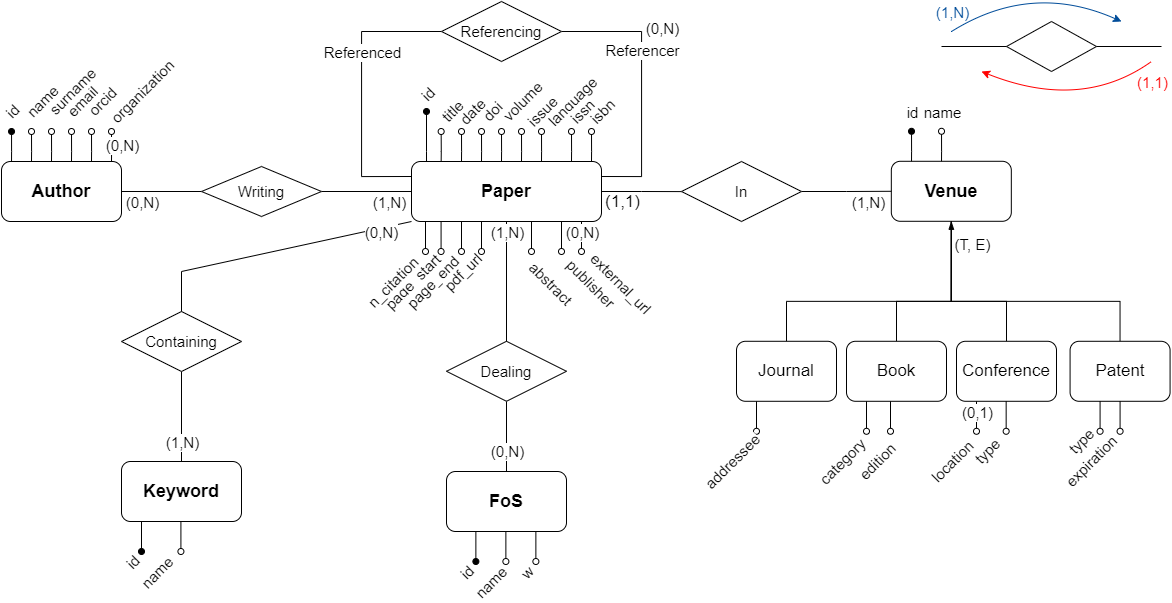
\includegraphics[width=1\textwidth]{Images/er_diagram.png}
    \caption{ER Diagram}
    \label{fig:quadtree}
\end{figure}
\subsection{Data set description}
The data set that was chosen for the goal of the project contains 8335 papers, 730 venues, 27576 authors and 25005 field of studies. It is a reduced version of the more complex model on which the ER Diagram is based. In fact, it doesn't contain the entities Keyword and the sub-entities Journal, Book, Conference and Patent that, instead, are transformed into an attribute of the entity Paper that is called doc\_type. All the respective attributes of these entities are eliminated. Moreover, the attribute \textit{date} of the Paper, that is generalized in the ER Diagram, becomes the year. Furthermore, in the reduced version of the data set, the relationship Referencing becomes a list of string that are the references of the Paper. Lastly, the chosen data set contains just the more significant attributes. 
Summarizing, the chosen data set is composed by the following entities and attributes:
\begin{itemize}
    \item \textbf{Paper} with the attributes: id (integer type), title (string type), year (integer type), n\_citation (integer type), page\_start (integer type), page\_end (integer type), doc\_type (string type), publisher (string type), volume (integer type), issue (integer type), doi (string type), references (list of string type), abstract (string type);
    \item \textbf{Author} with the attributes: paper\_id (integer type), author\_name (string type), author\_id (integer type), author\_org (string type);
    \item \textbf{FoS} with the attributes: paper\_id (integer type), fos\_name (string type), fos\_weight (float type);
    \item \textbf{Venue} with the attributes: paper\_id (integer type), venue\_name (string type), venue\_id (integer type).
\end{itemize}
\subsection{Data Pre-Processing}
The original data set can be downloaded \href{https://lfs.aminer.cn/misc/dblp.v11.zip}{\textit{here}}. 
Given that such data set was unnecessarily large for our purpose, we decided to reduce its size. We could have just cut it at a certain point, however we decided that it was better to work with consistent data, therefore we decided to carefully perform sub-sampling in an intelligent way. Such pre-processing was performed using multiple Python scripts and the \href{https://pandas.pydata.org/}{Pandas library}. 

Here we provide a description of all the scripts used, together with the procedure to obtain the final data set starting from the initial one. All of these scripts can be found in the \textit{scripts} folder of the \textit{neo4j} section of the \href{https://github.com/albertopirillo/smbud-project-2022}{\textit{GitHub repository}} of the project.

The notebook \textbf{dataset\_exploration.ipynb} contains a short description of every operation for explanatory reasons. This notebook processes only a small chunk of the data set. The same operations are performed on the whole data set in the script \textbf{dataset} \textbf{\_preprocessing.py.}

Here is a summary of the operations performed:
\begin{itemize}
    \item Removal of samples with Null and NaN values
    \item Removal of samples with an empty string in a field
\end{itemize}

The operations above are required to work with consistent data. Notice that we can afford to simply drop the samples that do not respect such conditions since we dispose of a very large data set.

The following operations are not required but were performed to reduce even further the size of the data set, with the objective of keeping only the "most important" samples. 

We kept the samples:
\begin{itemize}
    \item With a number of citations greater than a threshold
    \item With a reference count greater than a threshold
\end{itemize}

We converted the \textit{indexed\_abstract} field from an inverted index to a string of text, to make it easier to query once inserted into the database. The field was also renamed to \textit{abstract}.

We also processed the data set in order to remove some special characters not supported by the import function of the database. An example of such characters is "{\textbackslash}". This operation is performed in the script \textbf{remove\_special\_characters.py}.

Given that many samples were removed from the data set, we also had to fix up the \textit{references} field to keep only the valid ones. We consider a reference valid when it points to a sample of the data set that was kept. Otherwise, we say that such reference is invalid and we remove it from the data set. This operation is performed in the script \textbf{deprecated\_references.py}.

Lastly, when importing the data into the database, we realized that it was more practical to split the data set into multiple data sets to speed up the process and to produce cleaner code.  This functionality was added in the \textbf{dataset\_preprocessing.py} script. We split the data set following the structure of ER diagram, ending up with one separate data set for each entity present in the original data set. Thus, we ended up with 4 data sets: \textbf{Paper}, \textbf{Author}, \textbf{Venue} and \textbf{Fos}.

To obtain the final data set starting from the downloaded one, run the scripts in this order:

\begin{enumerate}
    \item \textbf{dataset\_preprocessing.py}
    \item \textbf{deprecated\_references.py}
    \item \textbf{remove\_special\_characters.py}
\end{enumerate}

The input of the first script is the initial data set. Only the paper data set requires to be processed by the second script, then only the paper and the venue data sets require to be processed by the third script. 
At the end, you will obtain 4 data sets which are identical to the ones that we imported into the database.

\section{Neo4j}
\label{ch:neo}
\subsection{Data Upload}
To import the data into Neo4j, there is one last precaution needed: it is necessary to process the Paper data set to make the \textit{references} field compatible with the import function of the database. To perform such action the script \textbf{preprocessing.py} can be used. The script is located in the \textit{neo4j} folder of the \href{https://github.com/albertopirillo/smbud-project-2022}{\textit{GitHub repository}}.
Now, the data sets can be correctly imported into the Neo4J database. In order to do that, you need to put the four data sets files in the program's import folder. 

Thanks to the pre-processing that was performed, the four data sets are saved in the simple CSV format and it is possible to use the LOAD CSV command to easily load all the entities and relationships.

\begin{enumerate}
    \item Clear the Database: \lstinputlisting[language=SQL]{code/data creation/Clean.txt}
    \item Load the Papers: \lstinputlisting[language=SQL]{code/data creation/Paper.txt}
    \item Load the Authors: \lstinputlisting[language=SQL]{code/data creation/Author.txt}
    \item Load the Fos: \lstinputlisting[language=SQL]{code/data creation/Fos.txt}
    \item Load the Venue: \lstinputlisting[language=SQL]{code/data creation/Venue.txt}
    \item Create the \verb |Writing|  relationship between papers and authors:\lstinputlisting[language=SQL]{code/data creation/Writing.txt}
    \item Create the \verb |Referring| relationship between papers and papers:\lstinputlisting[language=SQL]{code/data creation/Refering.txt}
    \item Create the \verb |in| relationship between papers and venues:\lstinputlisting[language=SQL]{code/data creation/In.txt}
    \item Create the \verb |dealing| relationship between papers and FoS:\lstinputlisting[language=SQL]{code/data creation/Dealing.txt}
\end{enumerate}
\newpage

\subsection{Graph Diagram}
Entities:
 \begin{figure}[H]
    \centering
     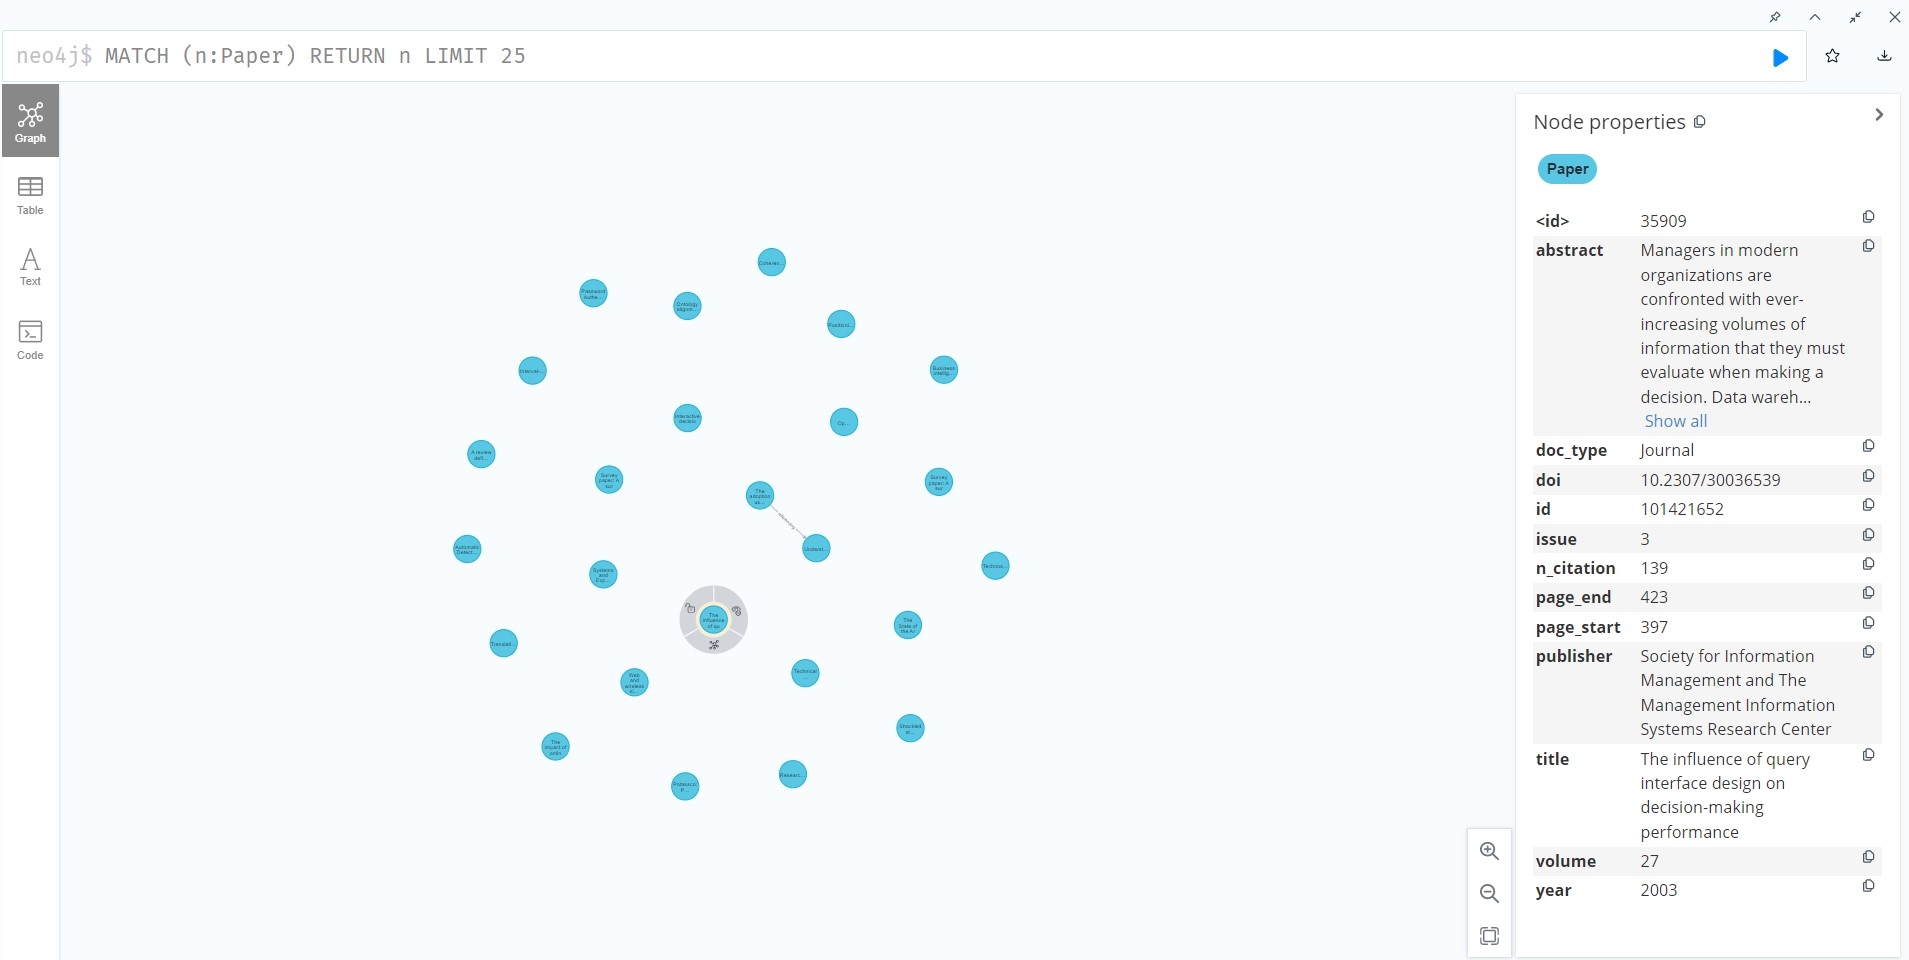
\includegraphics[width=0.8\textwidth]{Images/data/Paper.jpg}
    \caption{Paper}
    \label{fig:quadtree}
\end{figure}
    \begin{figure}[H]
    \centering
    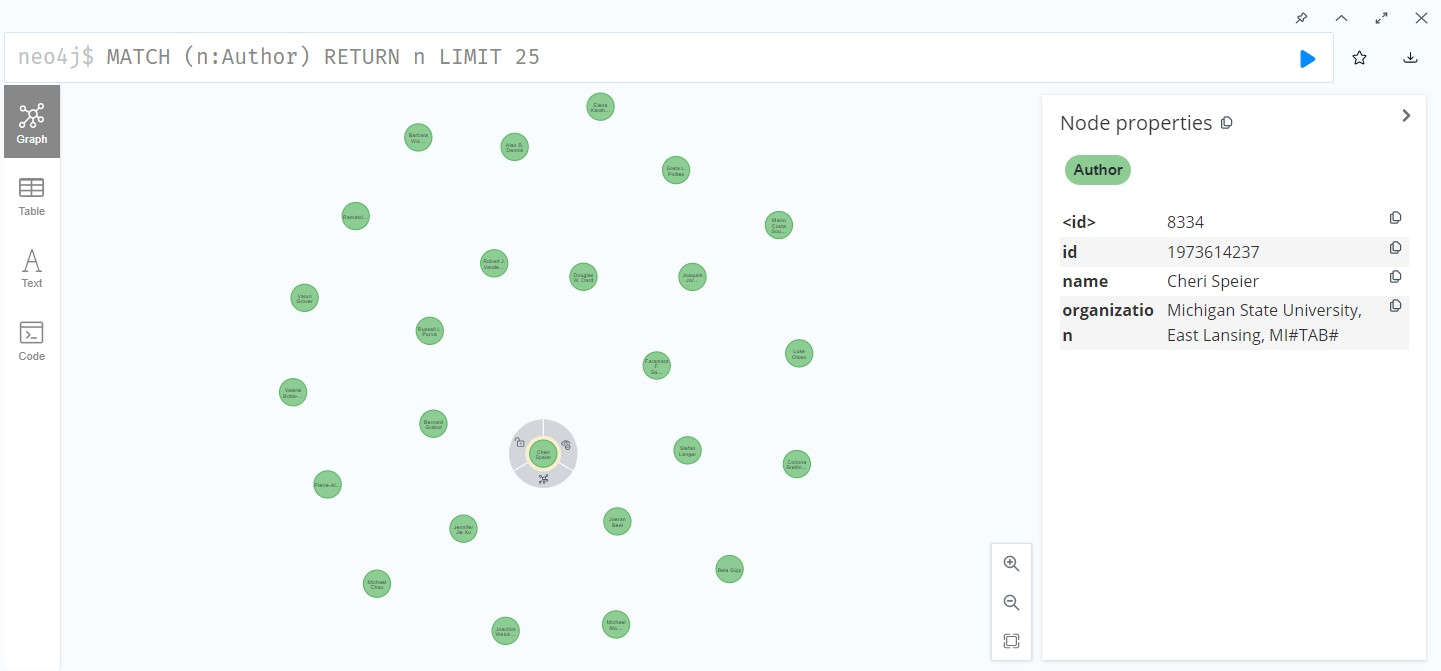
\includegraphics[width=0.8\textwidth]{Images/data/Author.jpg}
    \caption{Author}
    \label{fig:quadtree}
\end{figure}
\begin{figure}[H]
    \centering
    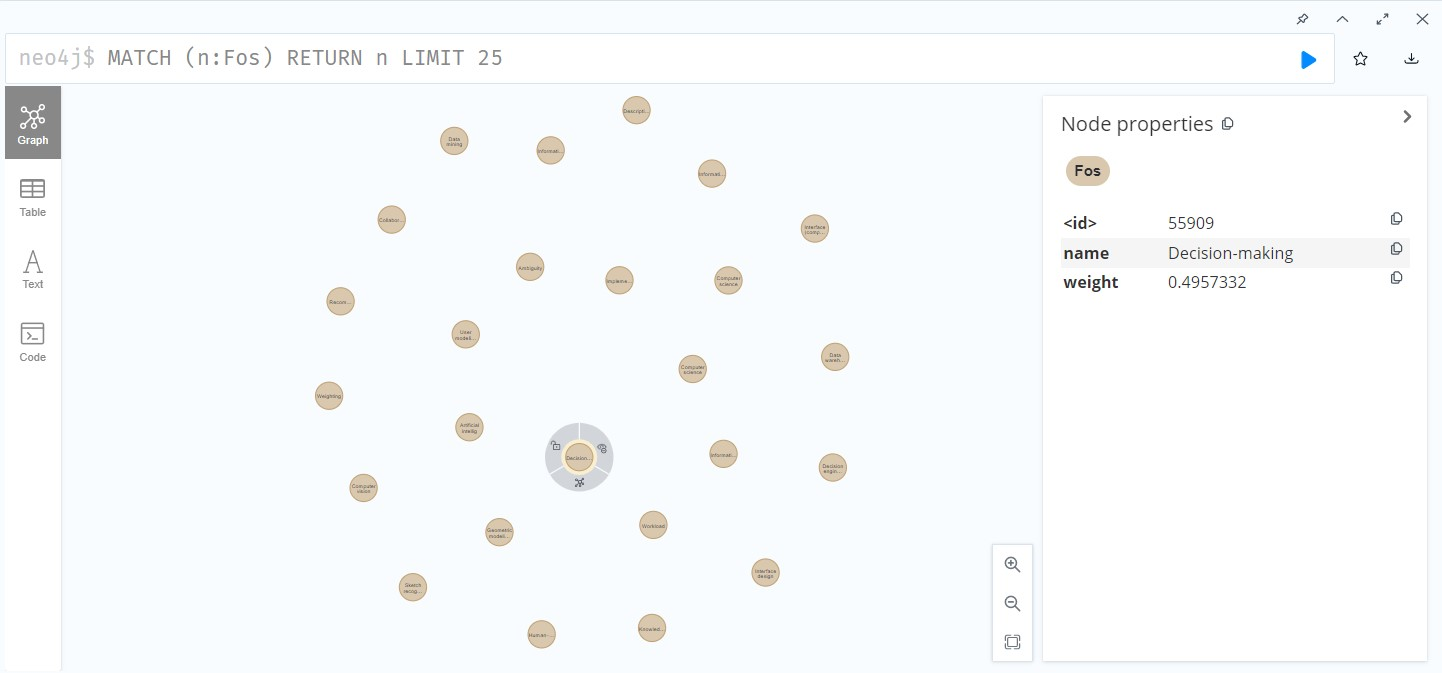
\includegraphics[width=0.8\textwidth]{Images/data/Fos.jpg}
    \caption{FoS}
    \label{fig:quadtree}
\end{figure}
\begin{figure}[H]
    \centering
    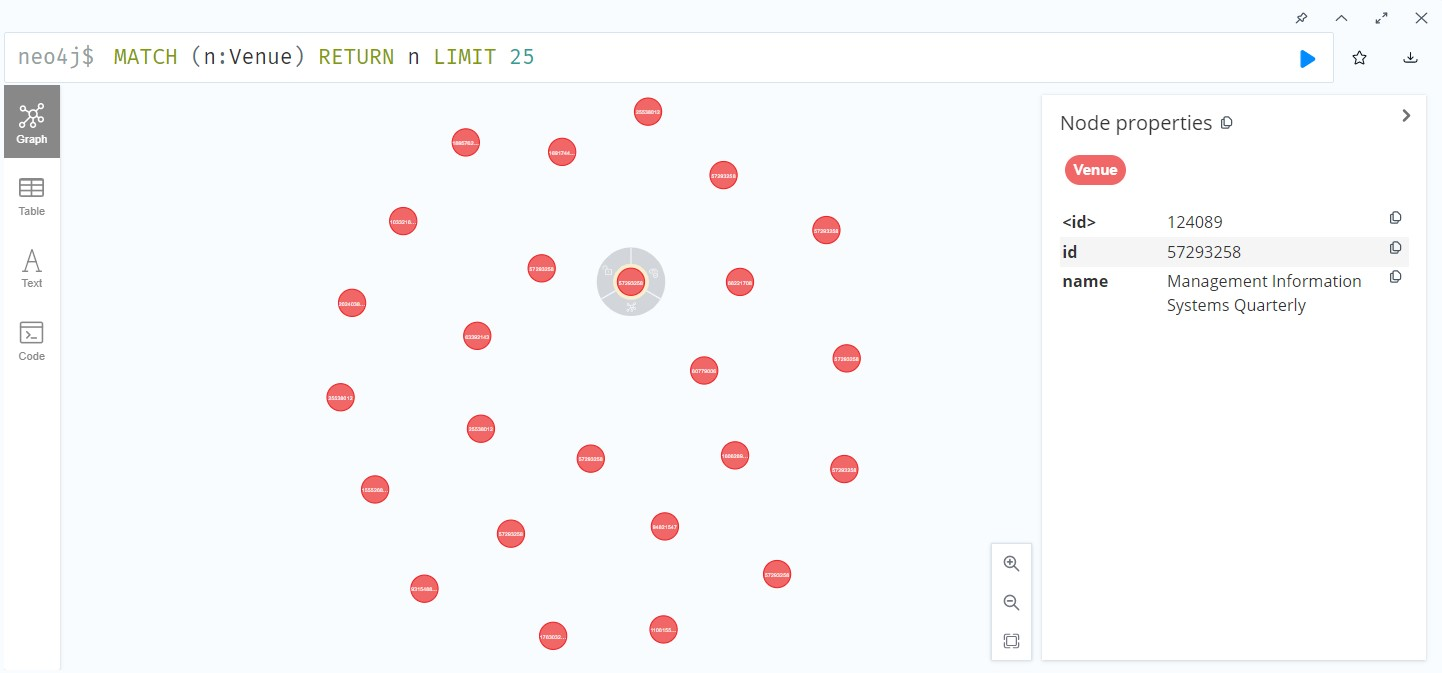
\includegraphics[width=0.8\textwidth]{Images/data/Venue.jpg}
    \caption{Venue}
    \label{fig:quadtree}
\end{figure}
  
Relationships:
    \begin{figure}[H]
    \centering
    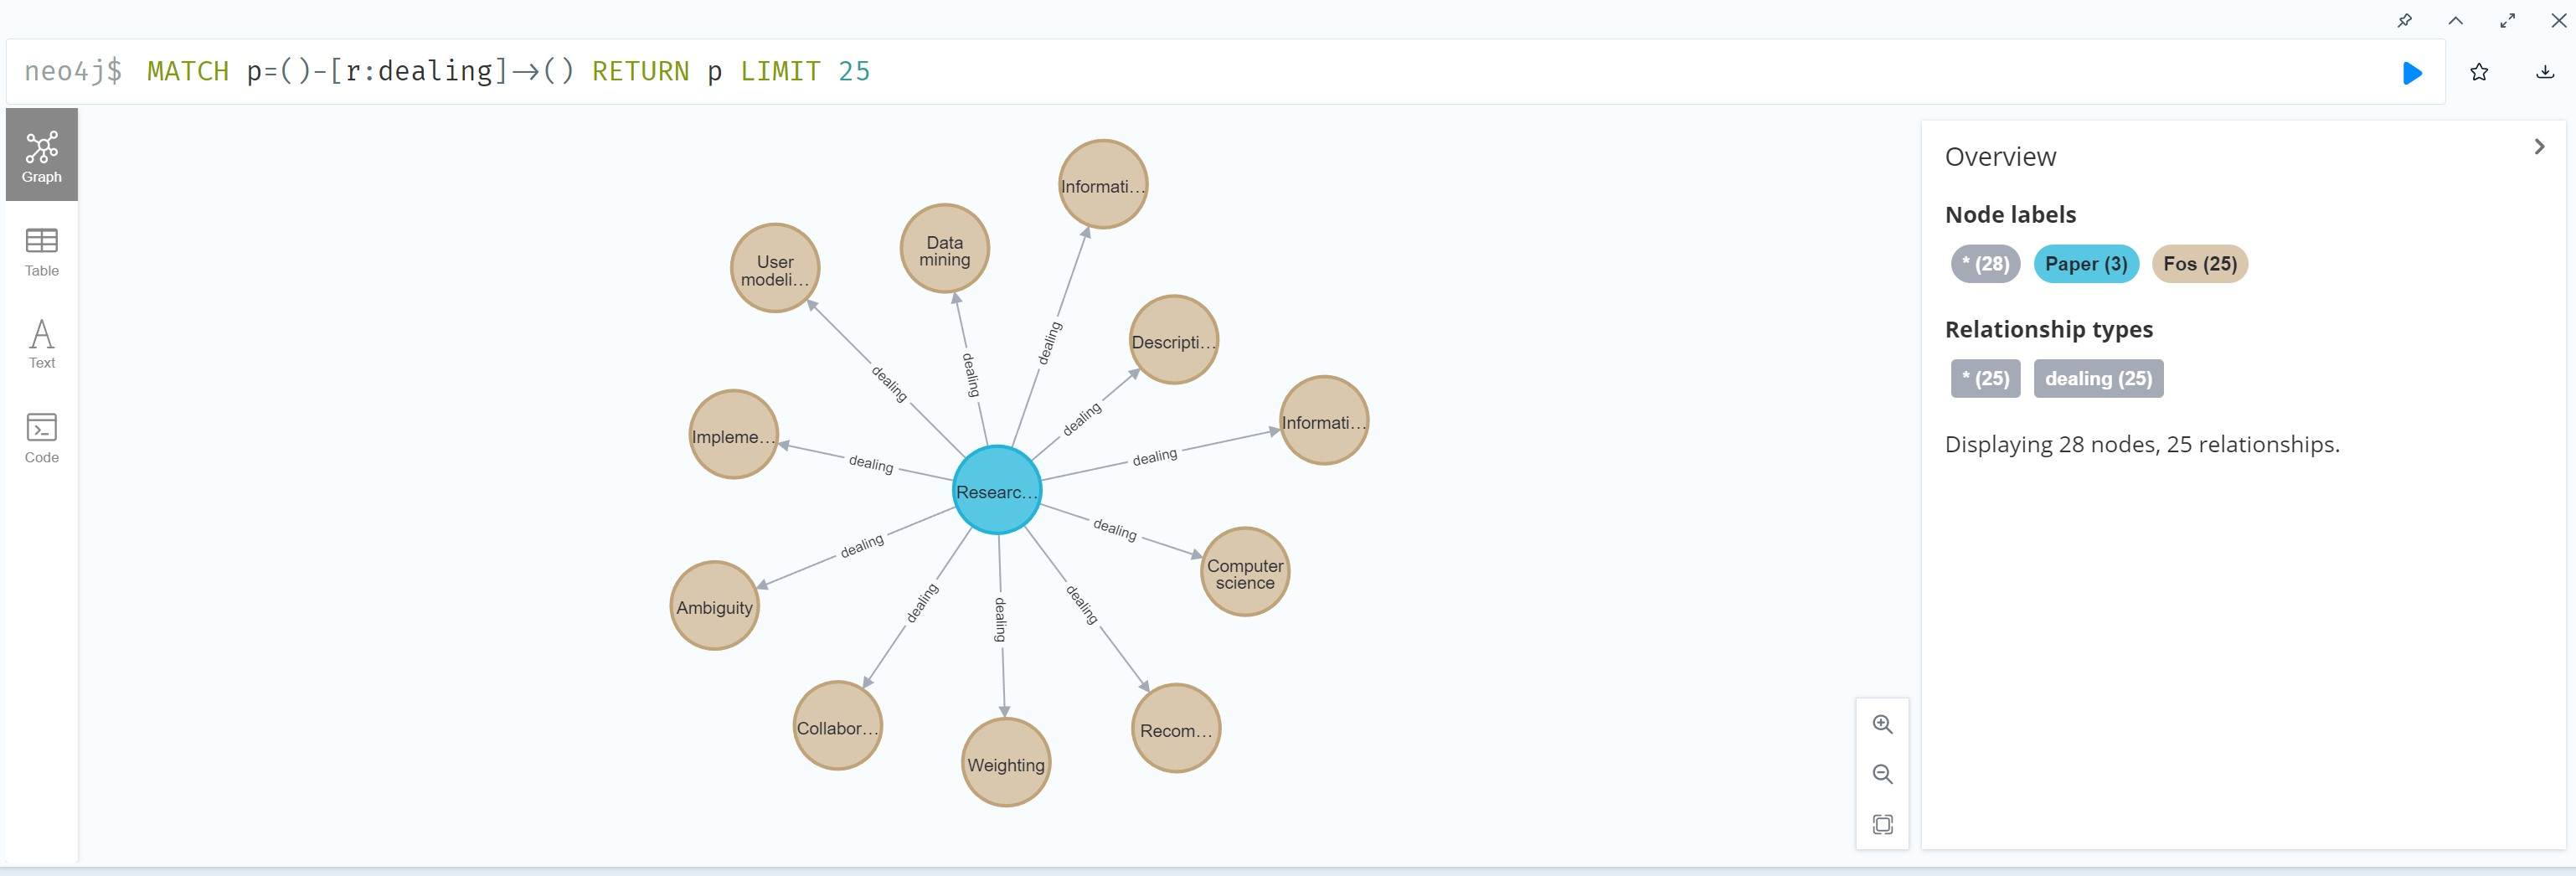
\includegraphics[width=0.8\textwidth]{Images/data/Dealing.jpg}
    \caption{Paper-Dealing->FoS}
    \label{fig:quadtree}
\end{figure}
 \begin{figure}[H]
    \centering
    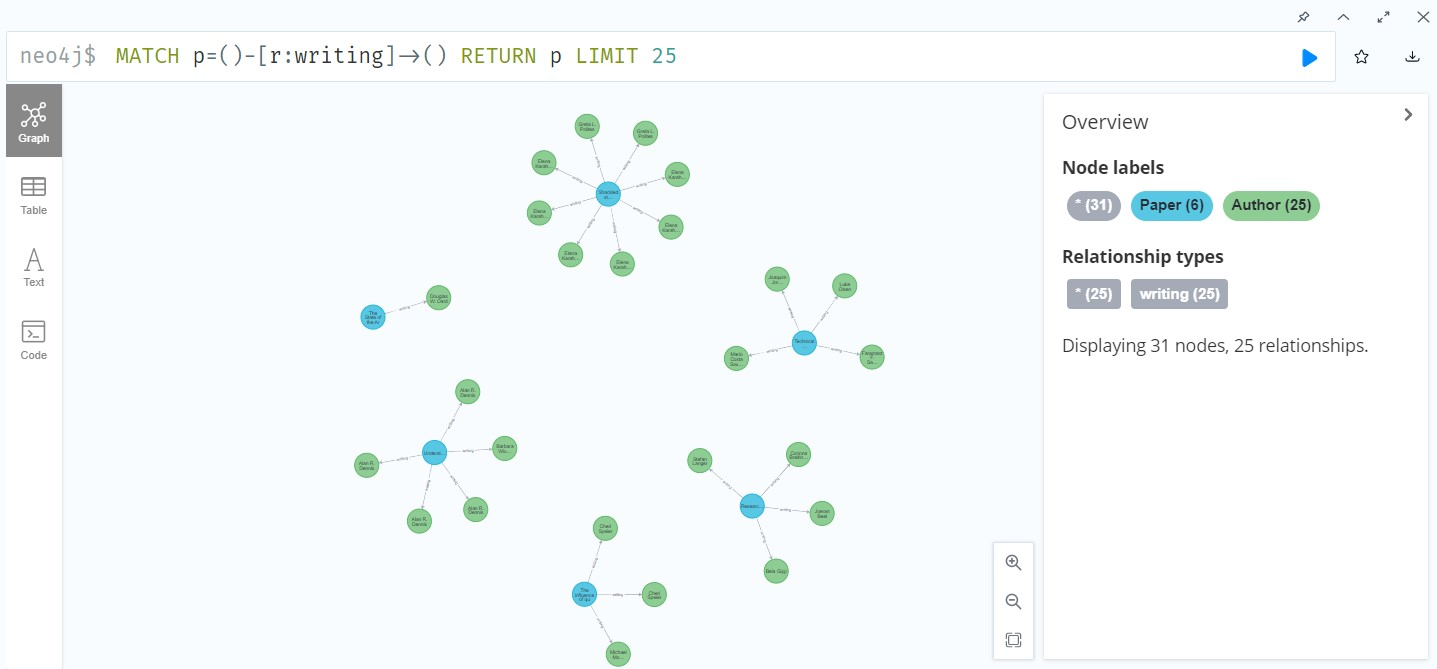
\includegraphics[width=0.8\textwidth]{Images/data/Writing.jpg}
    \caption{Paper-Writing->Author}
    \label{fig:quadtree}
\end{figure}
 \begin{figure}[H]
    \centering
    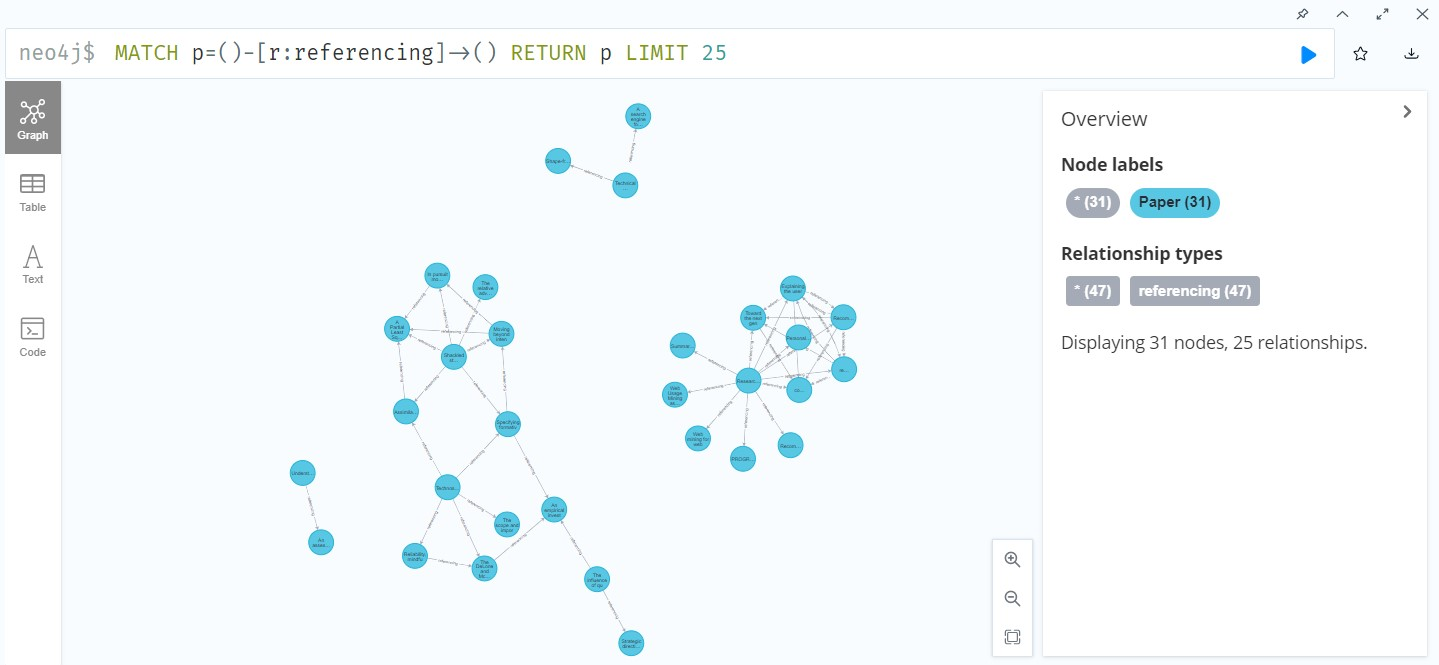
\includegraphics[width=0.8\textwidth]{Images/data/Referencing.jpg}
    \caption{Paper-Referencing->Paper}
    \label{fig:quadtree}
\end{figure}
\begin{figure}[H]
    \centering
    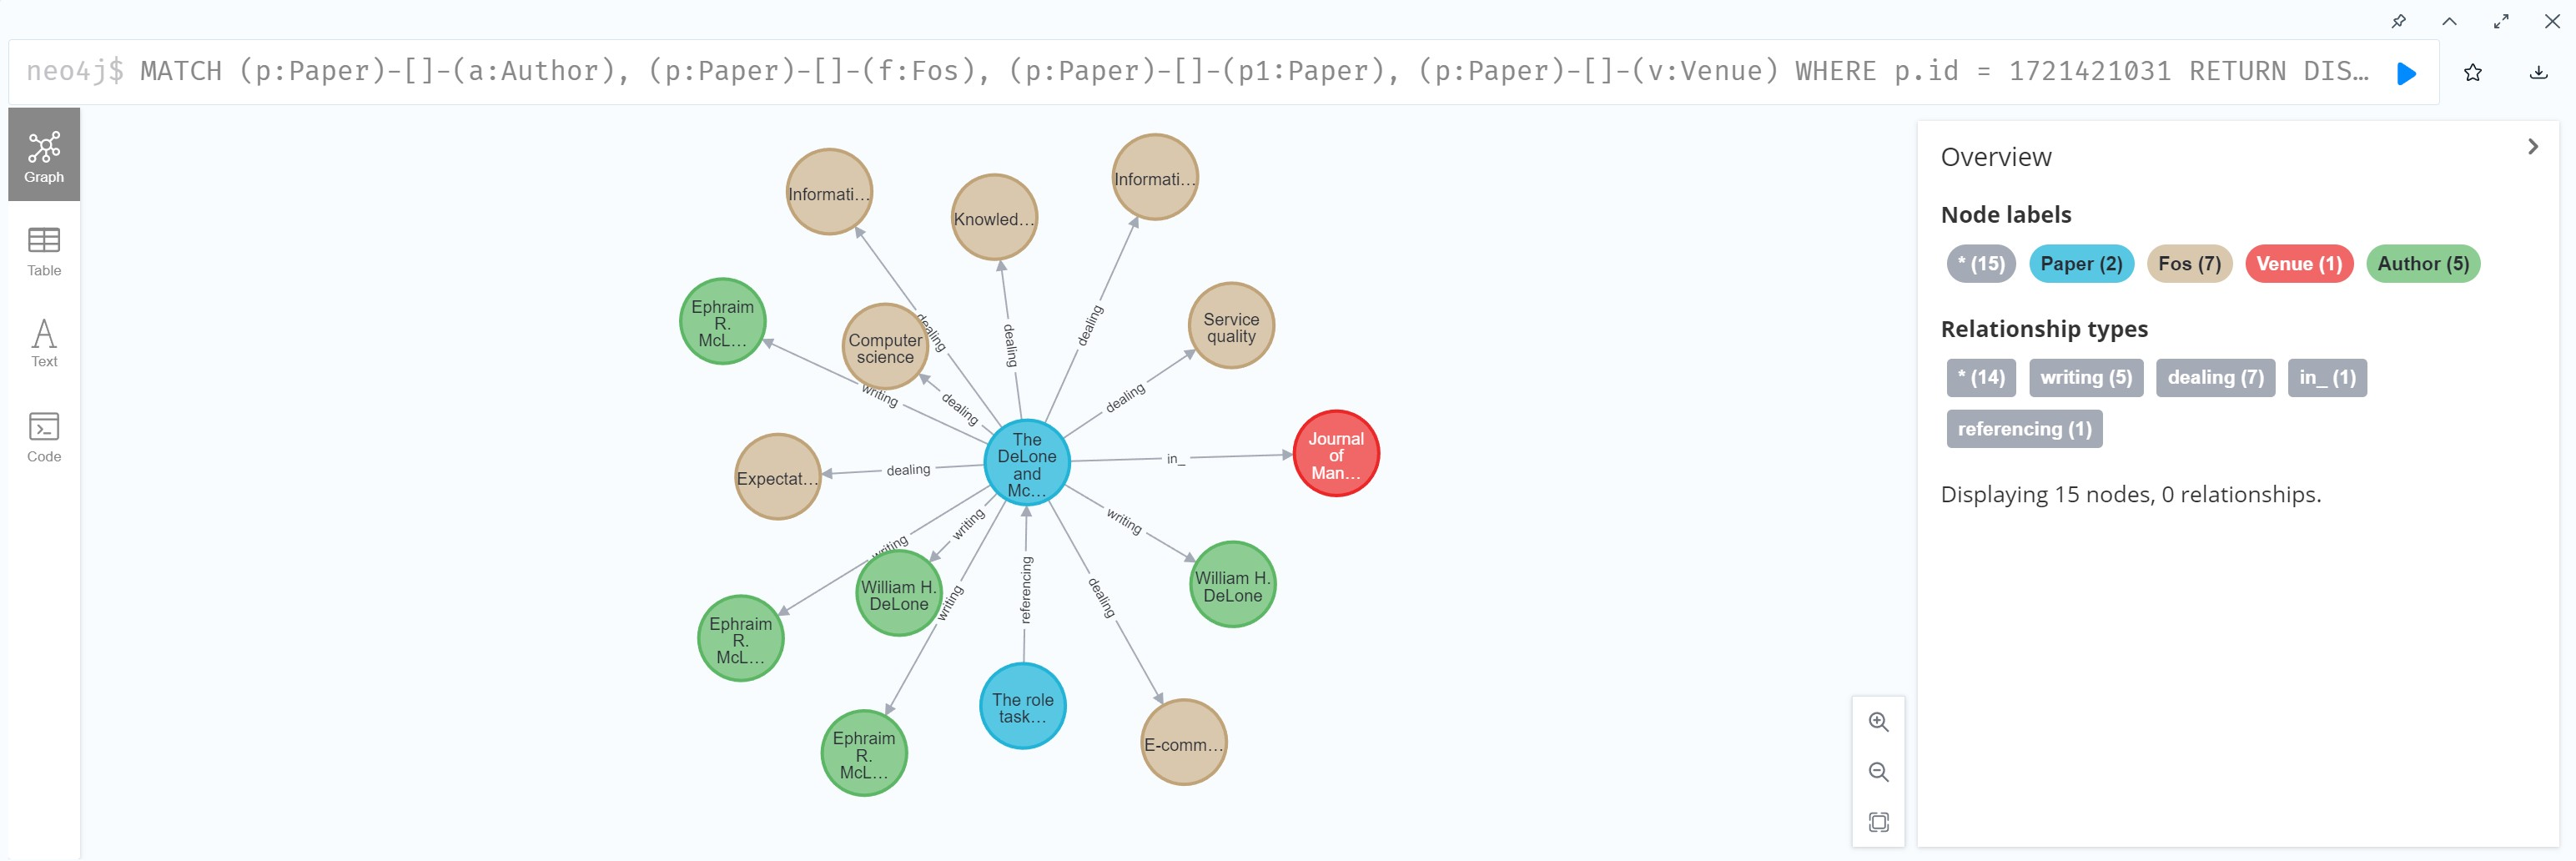
\includegraphics[width=0.8\textwidth]{Images/data/All_nodes_and_relations.jpg}
    \caption{All the relationships}
    \label{fig:quadtree}
\end{figure}

\subsection{Queries}
\begin{enumerate}
    \item \textbf{Find papers of a determined venue, written after a certain date (Execution time 454ms)}:
    \lstinputlisting[language=SQL]{code/queries_neo4j/query_1.txt}
     \begin{figure}[H]
    \centering
    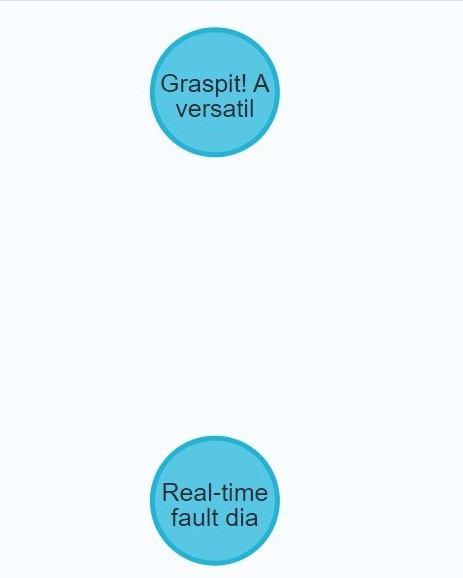
\includegraphics[width=0.4\textwidth]{Images/queries_neo4j/query_1.jpg}\end{figure}
    \item \textbf{Find papers in a set of venues, with a determined type (Execution time 2ms)}:
    \lstinputlisting[language=SQL]{code/queries_neo4j/query_2.txt}
     \begin{figure}[H]
    \centering
    
\includegraphics[width=0.7\textwidth]{Images/queries_neo4j/query_2.jpg}
    \end{figure}
  Below we can see the output of the profile statement, that is used to track the query and the numbers of rows of each operation. It starts by scanning all the nodes with the papers, then it expands all the nodes with the 'writing' relationship on the left of the picture and the 'in' relationship on the right. Finally, it applies the filters on the venue id and on the paper's doc type and returns the results.
    \begin{figure}[H]
    \centering
    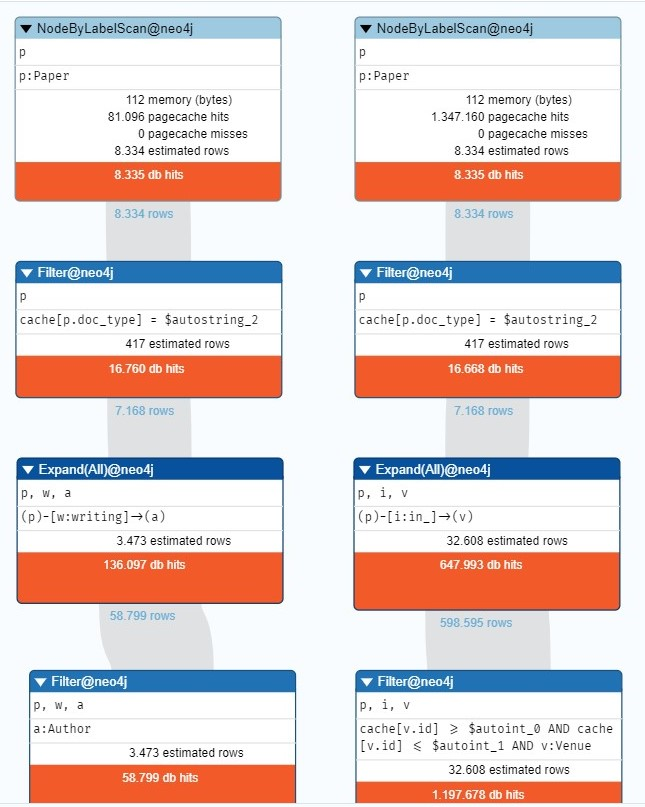
\includegraphics[width=0.5\textwidth]{Images/queries_neo4j/query_2_p1.jpg}
    \end{figure}
    \begin{figure}[H]
    \centering
    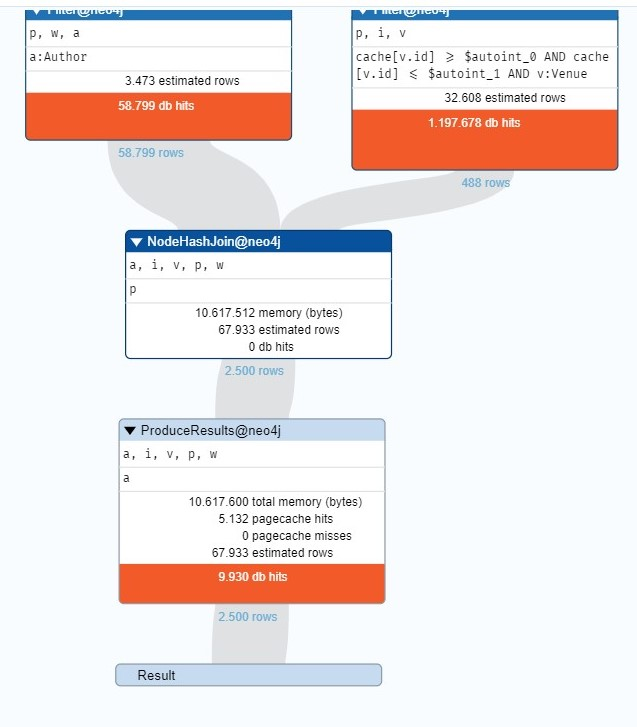
\includegraphics[width=0.5\textwidth]{Images/queries_neo4j/query_2_p2.jpg}
    \end{figure}
    \item \textbf{Find papers of a determined main argument, written after a certain date (Execution time 30ms)}:
    \lstinputlisting[language=SQL]{code/queries_neo4j/query_3.txt}
    \begin{figure}[H]
    \centering
    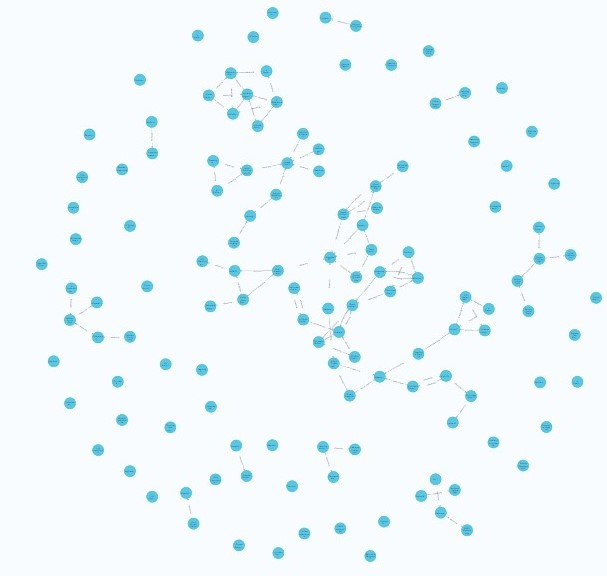
\includegraphics[width=0.4\textwidth]{Images/queries_neo4j/query_3.jpg}
    \end{figure}
    \item \textbf{Count the authors that have written a famous paper of a determined argument (Execution time 38ms)}:
    \begin{figure}[H]
    \centering
    \lstinputlisting[language=SQL]{code/queries_neo4j/query_4.txt}
    \end{figure}
    \begin{figure}[H]
    \centering
    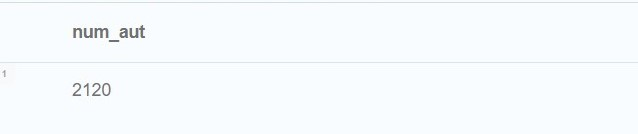
\includegraphics[width=\textwidth]{Images/queries_neo4j/query_4.jpg}
    \end{figure}
    \item \textbf{Count the papers divided per author written in a set of venue by a determined authors' organization (Execution time 103ms)}:
    \lstinputlisting[language=SQL]{code/queries_neo4j/query_5.txt}
    \begin{figure}[H]
    \centering
    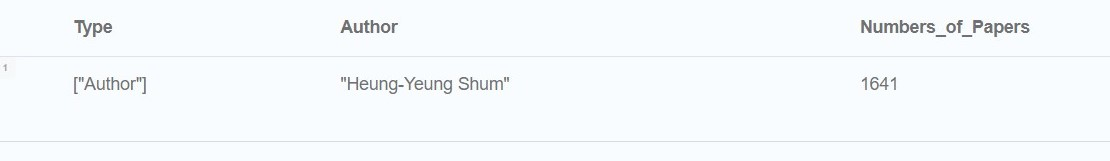
\includegraphics[width=\textwidth]{Images/queries_neo4j/query_5.jpg}
    \end{figure}
  The profile statement scans all the authors, then it expands the 'writing' relationship and applies the organization's filter. At the same time it scans all the venues and filters their id. At the end the aggregation is applied and all the resulting values are returned.
    \begin{figure}[H]
    \centering
    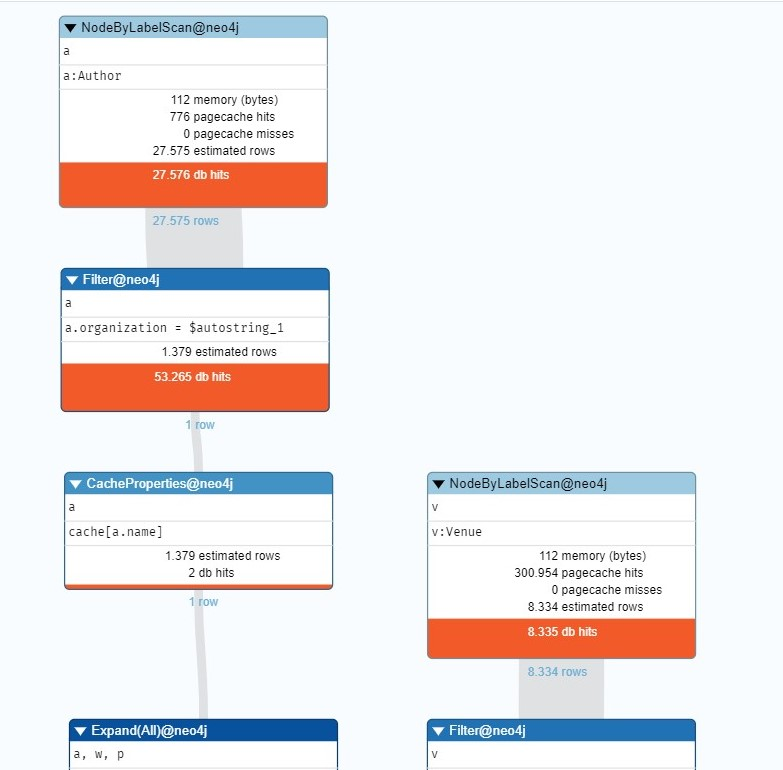
\includegraphics[width=0.5\textwidth]{Images/queries_neo4j/query_5_p1.jpg}
    \end{figure}
    \begin{figure}[H]
    \centering
    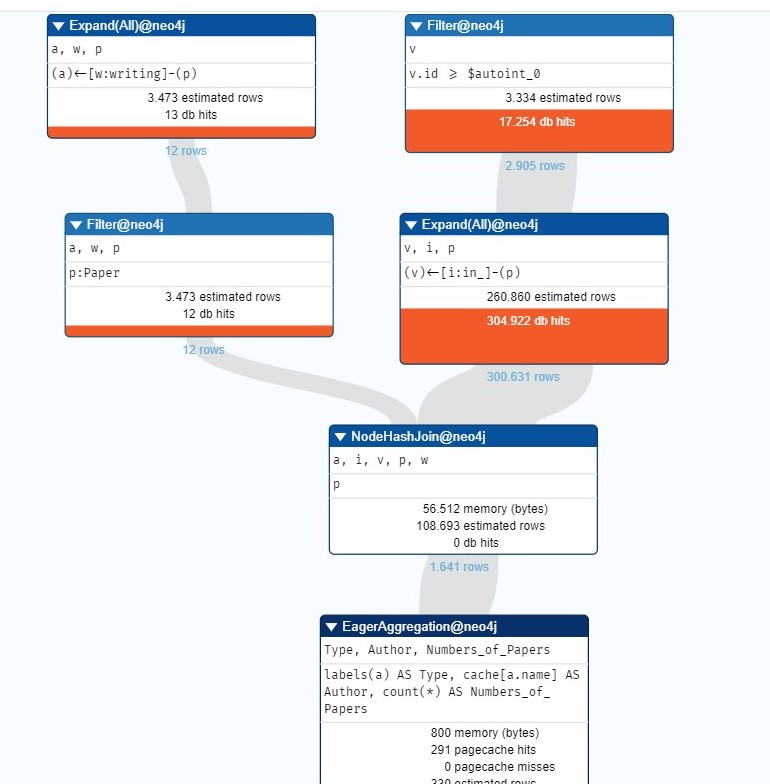
\includegraphics[width=0.5\textwidth]{Images/queries_neo4j/query_5_p2.jpg}
    \end{figure}
    \begin{figure}[H]
    \centering
    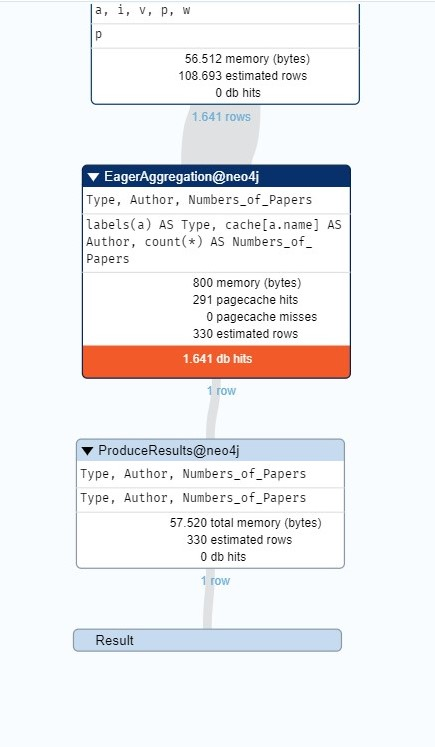
\includegraphics[width=0.5\textwidth]{Images/queries_neo4j/query_5_p3.jpg}
    \end{figure}
     \item \textbf{Calculate the weight keywords' average of papers that have a determined publisher and a reference to a famous paper  (Execution time 27ms)}:
    \lstinputlisting[language=SQL]{code/queries_neo4j/query_6.txt}
    \begin{figure}[H]
    \centering
    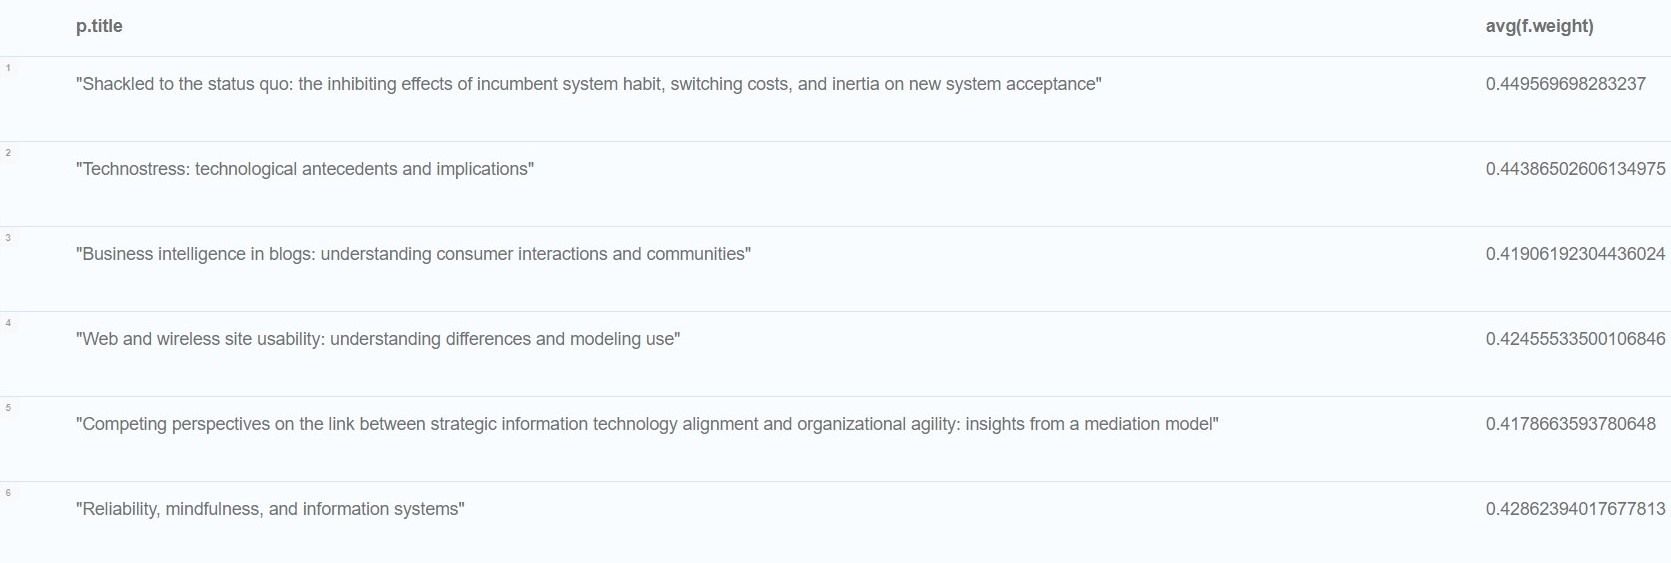
\includegraphics[width=\textwidth]{Images/queries_neo4j/query_6.jpg}
    \end{figure}
    \item \textbf{Count the numbers of bilateral reference between two papers that have the same venue and a large  number of citation (Execution time 119ms)}:
    \lstinputlisting[language=SQL]{code/queries_neo4j/query_7.txt}
    \begin{figure}[H]
    \centering
    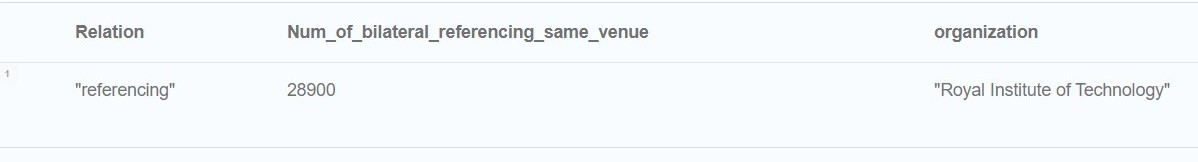
\includegraphics[width=\textwidth]{Images/queries_neo4j/query_7.jpg}
    \end{figure}
    \item \textbf{Count the total citation of a paper that have references to two papers that deal of different field of study (Execution time 1849ms)}:
    \lstinputlisting[language=SQL]{code/queries_neo4j/query_8.txt}
    \begin{figure}[H]
    \centering
    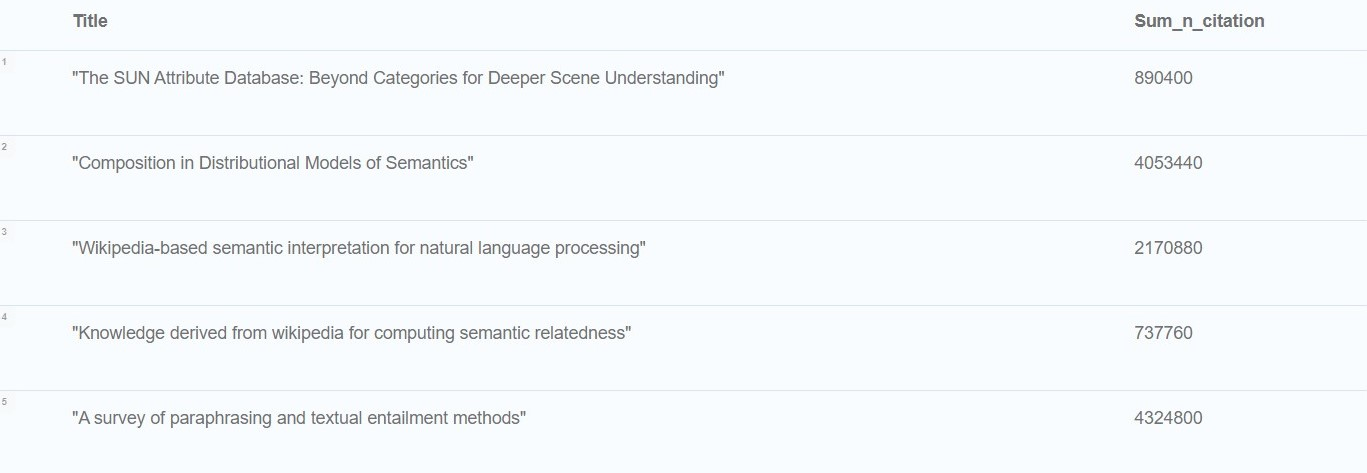
\includegraphics[width=\textwidth]{Images/queries_neo4j/query_8.jpg}
    \end{figure}
    \item \textbf{Find the shortest path between two different paper that have a reference in common where the first is less famous than the second one (Execution time 61ms)}:
    \lstinputlisting[language=SQL]{code/queries_neo4j/query_9.txt}
    \begin{figure}[H]
    \centering
    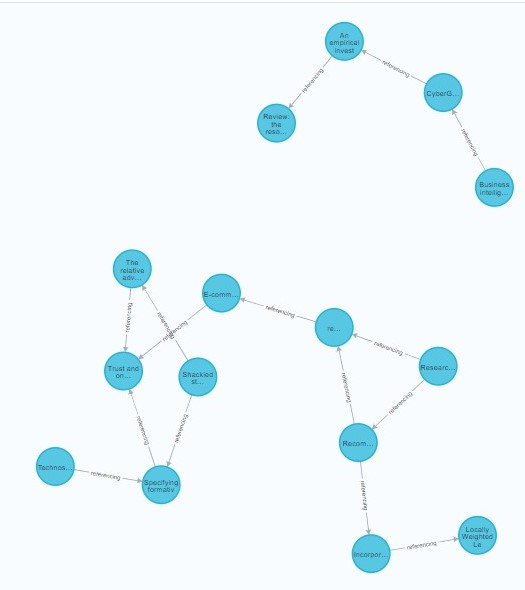
\includegraphics[width=0.5\textwidth]{Images/queries_neo4j/query_9.jpg}
    \end{figure}
    \newpage
    \item \textbf{Find the shortest path between two different paper that have a reference in common different FoS (Execution time 42ms)}:
    \lstinputlisting[language=SQL]{code/queries_neo4j/query_10.txt}
    \begin{figure}[H]
    \centering
    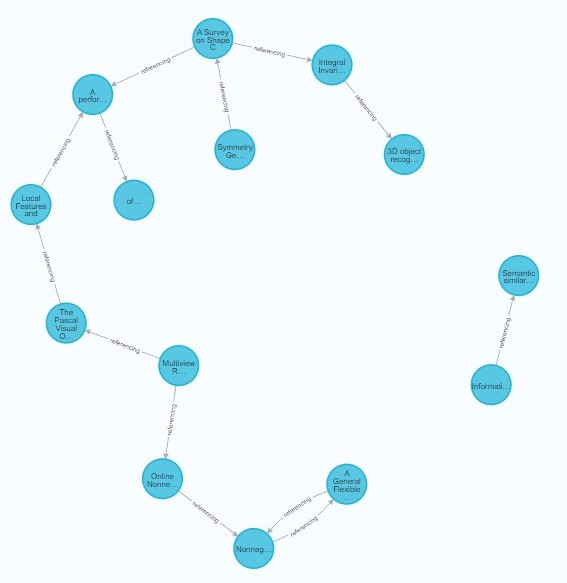
\includegraphics[width=0.4\textwidth]{Images/queries_neo4j/query_10.jpg}
    \end{figure}
  In the following page we can see that the profile statement scans the FoS, applies the filters to them and expands the 'dealing' relationship. Then it checks that paper1 and paper2 are different and in the end it calls the function 'shortestPath' and returns the results.
    \begin{figure}[H]
    \centering
    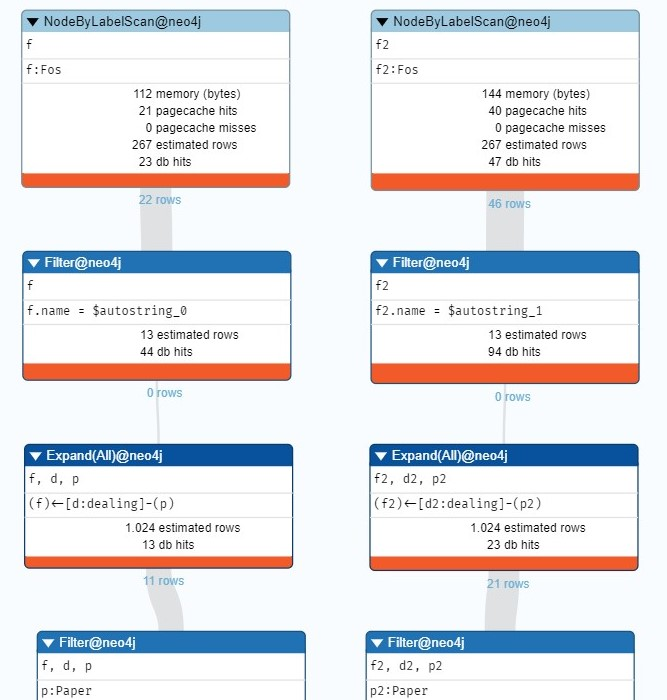
\includegraphics[width=0.5\textwidth]{Images/queries_neo4j/query_10_p1.jpg}
    \end{figure}
    \begin{figure}[H]
    \centering
    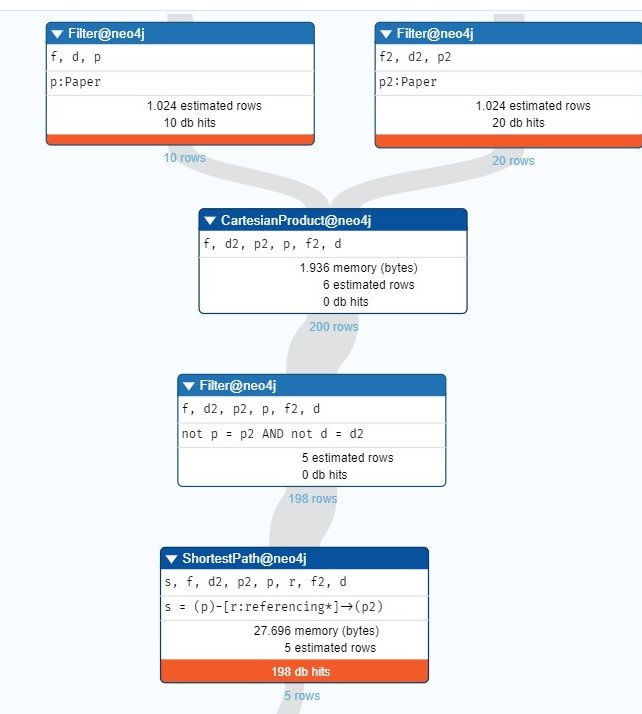
\includegraphics[width=0.5\textwidth]{Images/queries_neo4j/query_10_p2.jpg}
    \end{figure}
    \begin{figure}[H]
    \centering
     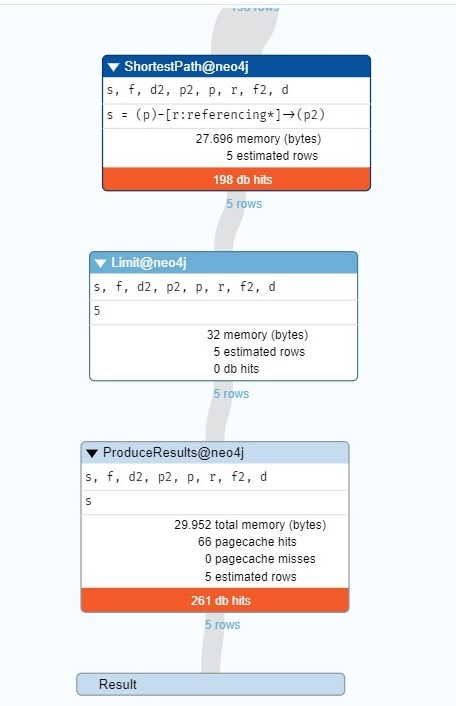
\includegraphics[width=0.5\textwidth]{Images/queries_neo4j/query_10_p3.jpg}
     \end{figure}
\end{enumerate}
\subsection{Creation/Update Commands}
\begin{enumerate}
\item \textbf{Insertion of a new author in the database}:
    \lstinputlisting[language=SQL]{code/commands_neo4j/cmd_1.txt}
\item \textbf{Insertion of a new field of study in the database}:
    \lstinputlisting[language=SQL]{code/commands_neo4j/cmd_2.txt}
\item \textbf{Insertion of a new venue in the database}:
    \lstinputlisting[language=SQL]{code/commands_neo4j/cmd_3.txt}
\item \textbf{Insertion of a new paper in the database, paper's relationships with authors, venue, fields of study and other papers are created}:
    \lstinputlisting[language=SQL]{code/commands_neo4j/cmd_4.txt}
\item \textbf{Update of the organization of an author}:
    \lstinputlisting[language=SQL]{code/commands_neo4j/cmd_5.txt}
\item \textbf{Update of the number of citations of a paper}:
    \lstinputlisting[language=SQL]{code/commands_neo4j/cmd_6.txt}
\end{enumerate}

\chapter{Second Delivery}

\section{Introduction}
\label{se:probdes1}
This project aims at building an Information System that manages a data set containing different type of scientific articles that can be used for: clustering with network and side information, studying influence in the citation network, finding the most influential papers and topics, modeling analysis.

For the same problem described in Chapter 1 (First Delivery), we modeled a different system following the subsequent steps.\\
At first the data set was pre-processed to add the fields that were missing in the original data set. Such fields were taken from different Kaggle data sets. 
Then it was reduced in size and after that it was uploaded on MongoDB.\\
At the end of the project 11 queries and 6 creation/update commands were initiated with a different level of complexity that was checked within the performance time.\\

\section{Data}
This is the structure of a paper inside the database, it contains different sub-documents: authors, fos (metadata), venue and sections.\\

\lstinputlisting[language=SQL]
{code/json/json.txt}
\label{json}

This is the description of a paper:\\
\textbf{Paper} is a scientific article that is associated with the following fields:
    \begin{itemize}
        \item \textit{id}: Int;
        \item \textit{title}: String;
        \item \textit{abstract}: that is the summary of the paper: String;
        \item \textit{authors}:
            \begin{itemize}
              \item \textit{name}: String;
              \item \textit{organization}: String;
               \item \textit{email}: that is a personal contact of the author: String;
               \item \textit{bio}: a short introduction written by the author (it is added from other sources): String;
            \end{itemize}
        \item \textit{FOS (Field of Study)}:
            \begin{itemize}
              \item \textit{name}: String;
              \item \textit{w}:  that is the weight of the fields of study: Float;
            \end{itemize}
        \item \textit{Publication Details}:
            \begin{itemize}
              \item \textit{year}: that corresponds to the publication year: Int;
              \item \textit{page\_start} and \textit{page\_end}: that are the starting and the ending point of the collection from which the paper was extracted: Int;
              \item \textit{doc\_type}: that is the type of the paper, and can assume 3 values: \textit{Journal}, \textit{Conference}, \textit{Patent}: String;
                \item \textit{publisher}: String;
              \item \textit{volume}: that corresponds to the n-th published collection: Int;
              \item \textit{issue}: that corresponds to the m-th part of the volume: Int;
               \item  \textit{doi}: that is the Digital Object Identifier: String;
              \item \textit{n\_citation}: that is the number of citations: Int;
            \end{itemize}
        \item \textit{Venue}: that is the collection from which the paper was extracted, with the attributes:
            \begin{itemize}
                \item \textit{id}: String;
                \item \textit{raw}: that is the name of the collection: String;
            \end{itemize}
        \item \textit{References}:
            \begin{itemize}
                \item \textit{id}: String;
            \end{itemize}
        \item \textit{Sections}: every section has an id, a title and a content (textual), it could have some subsections too (with the same structure of a section). Furthermore every section has one or more images. Every image has an url and a caption:
            \begin{itemize}
                \item \textit{id}: Int;
                \item \textit{title}: String;
                \item \textit{text}: String;
                \item \textit{subsections}:
                    \begin{itemize}
                        \item \textit{id}: Int;
                        \item \textit{title}: Int;
                        \item \textit{text}: String;
                    \end{itemize}
                \item \textit{figures}:
                    \begin{itemize}
                        \item \textit{url}: String;
                        \item \textit{caption}: String;
                    \end{itemize}
            \end{itemize}
            
        \end{itemize}

\subsection{Data Pre-Processing}
In this part of the project we used as a starting point the same data set used in the first delivery, which can be downloaded \href{https://lfs.aminer.cn/misc/dblp.v11.zip}{\textit{here}}. 
However, the pre-processing this time was slightly different. 
Roughly the same operations of the first delivery were performed to clean and reduce the size of the data set. Those operations are performed with the script \textbf{dataset\_preprocessing.py}, which can be found in the \textit{scripts} folder of the \textit{mongodb} section of the \href{https://github.com/albertopirillo/smbud-project-2022}{repository}.
It is worth to notice that such script does not split the original data set into multiple ones like in the first delivery. Instead, a single data set is kept.

\subsection{Data Completion}
We decided to avoid working with synthetic data (i.e. generate random meaningless data) and instead we decided to add to our dataset the missing field by retrieving data from other data sets, trying to be as accurate as possible. The missing field w.r.t. the description in section \ref{json} were:
\begin{itemize} 
    \item \textit{authors.email}
    \item \textit{authors.bio}
    \item \textit{sections}
\end{itemize}

We generated the email of every author and we inserted their bio, that were taken from Kaggle's Goodread-Authors data set. This is performed with the script \textbf{update\_author.py}.

Furthermore we added the \textit{Sections} part, using a  \href{https://transparency.twitter.com/en/reports/moderation-research.html}{Twitter dataset}, that contains millions of tweets in different languages. For every paper we generated randomly a number of sections in the range from 1 to 3 and for each one from 0 to 2 subsections. For the title we used the text of one tweet and for the content the text of four tweets.

Then for the figures we used another data set (Train-GCC-training.tsv from the Google Conceptual Captions official website) in order to take the \textit{image.url} and the \textit{image.caption} fields. Every section contains a random number of figures between 1 and 3.

Those two operations above are executed in the notebook \textbf{sections\_preprocessing.py}, that can be found in the \textit{mongodb} section of the \href{https://github.com/albertopirillo/smbud-project-2022}{GitHub repository}. 

The final data set consists of 8333 documents. 

To obtain the final data set starting from the downloaded one, run the scripts in this order:
\begin{enumerate} 
    \item \textbf{dataset\_preprocessing.py}
    \item \textbf{deprecated\_references.py}
    \item \textbf{bio\_preprocessing.py}
    \item \textbf{update\_author.py}
    \item \textbf{sections\_preprocessing.py}
\end{enumerate}

\pagebreak
\section{MongoDB}
\label{ch:mongo}
\subsection{Data Upload}
To import the data into a MongoDB collection, we rely on another Python script that exploits the \href{https://www.mongodb.com/docs/drivers/pymongo/}{PyMongo library}, the official MongoDB driver for Python.
We used the script \textbf{import\_data.py}, that can be found in the \textit{scripts} folder of the \textit{mongodb} section of the \href{https://github.com/albertopirillo/smbud-project-2022}{GitHub repository}. The script dumps the whole data set into a MongoDB collection, while preserving its complex and nested structure. It also performs some pre-processing on the \textit{id} and on the \textit{references} fields:
\begin{itemize}
    \item The \textit{id} field is renamed to \textit{\_id} in order to be used as an index inside of the database
    \item Both the \textit{\_id} field and the \textit{references} field are converted to an ObjectId.
\end{itemize}
Once the correct connection parameters and the correct file path have been specified, it is enough to run the script with Python to import the data. We will use \textit{papers} as the name of the collection.

\subsection{Document Example}
Below we can see the general structure of a document, with the help of \href{https://www.mongodb.com/products/compass}{MongoDB Compass}.
 \begin{figure}[H]
    \centering
    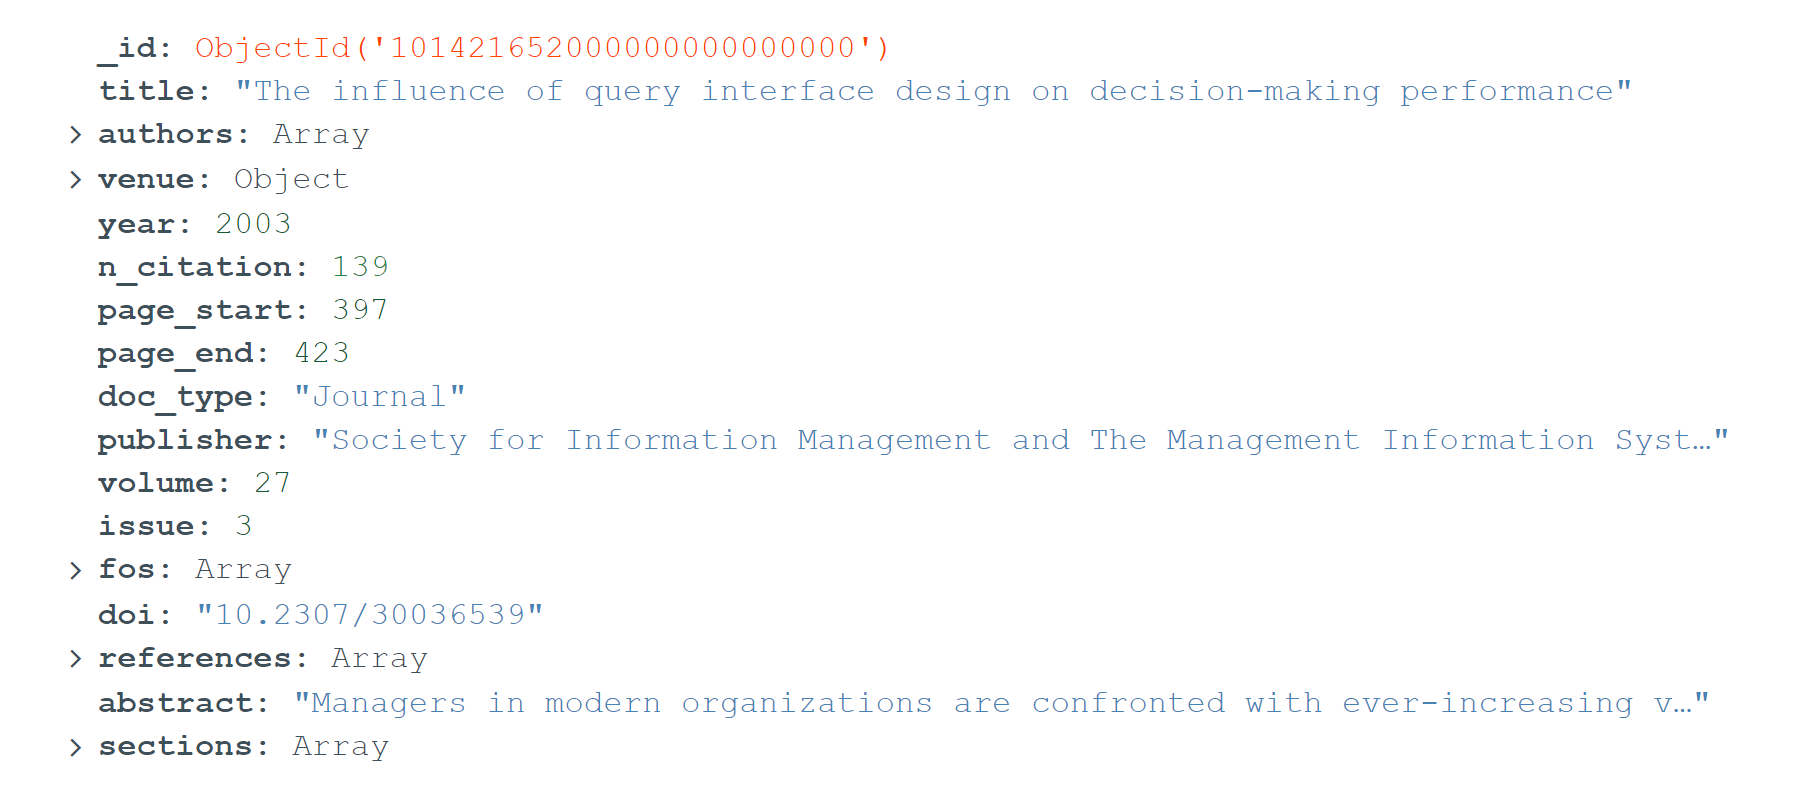
\includegraphics[width=\textwidth]{Images/data/mongodb/doc_general.png}
    \caption{General structure}
\end{figure}

\pagebreak
We will now expand the structure of the fields with a complex type. \\
The \textit{authors} field is an array of sub-documents in which every element represents an author that worked on the paper.
 \begin{figure}[H]
    \centering
    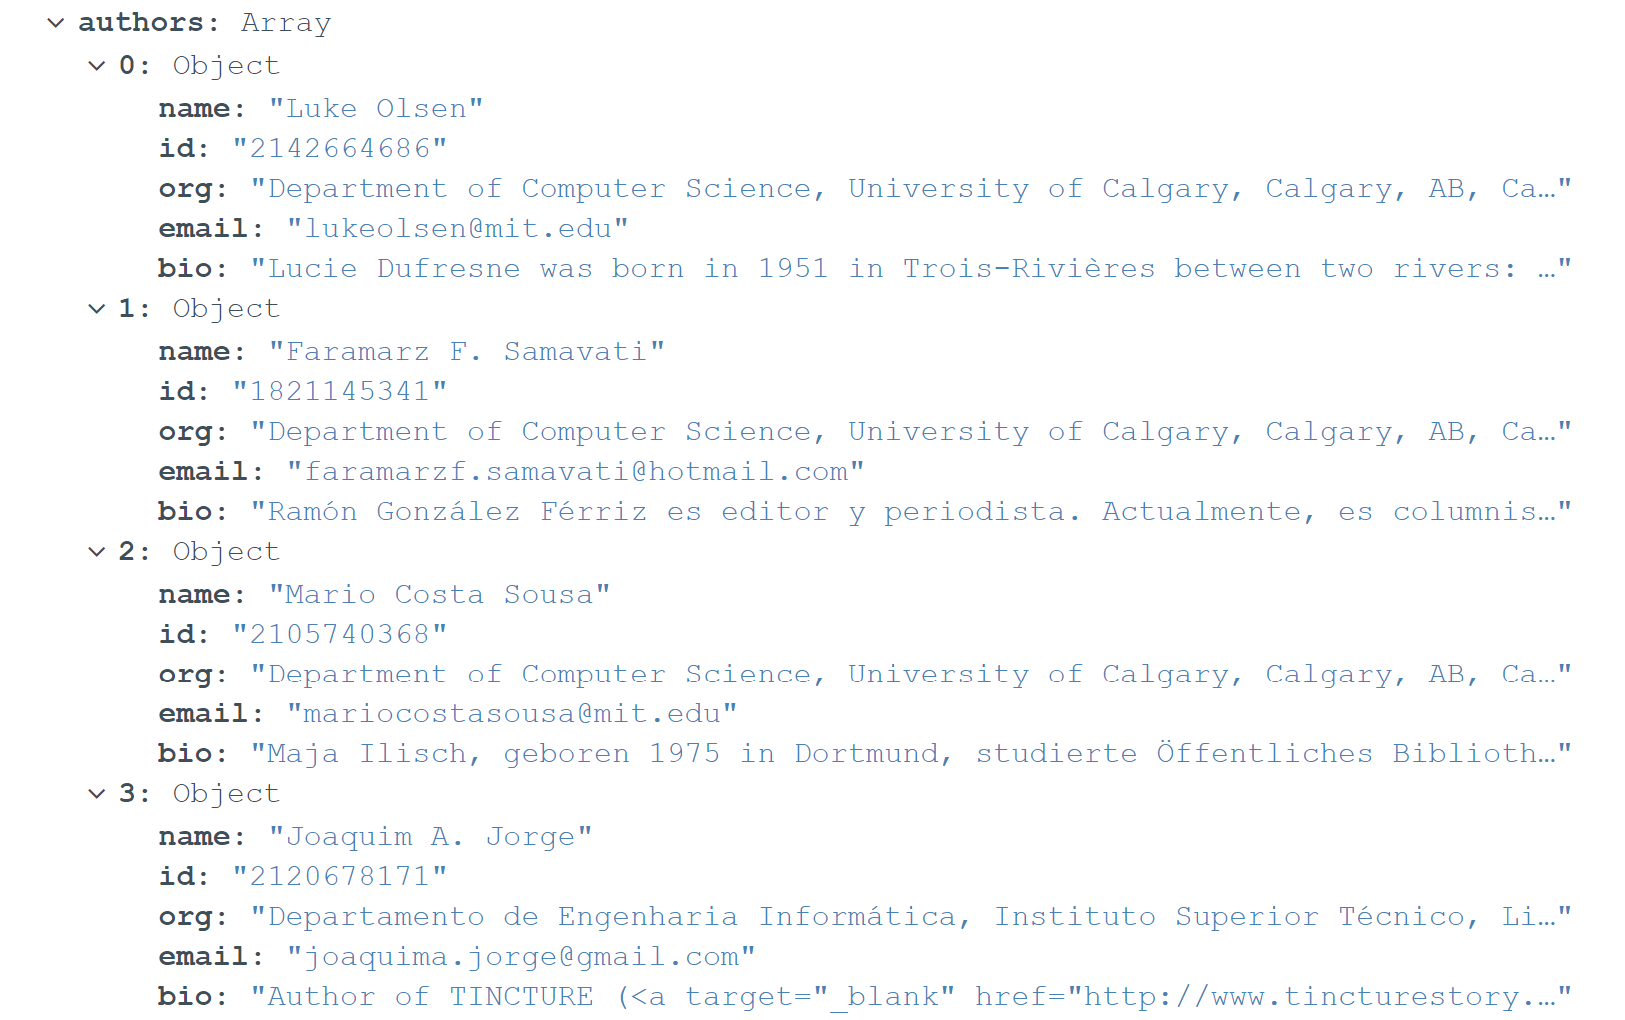
\includegraphics[width=0.9\textwidth]{Images/data/doc_authors.png}
    \caption{Structure of the \textit{authors} field}
\end{figure}

The \textit{venue} field is a sub-document with two internal fields.
 \begin{figure}[H]
    \centering
    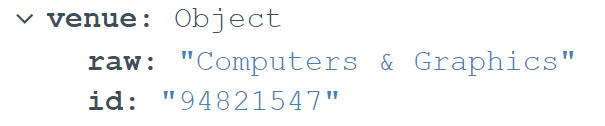
\includegraphics[width=0.5\textwidth]{Images/data/doc_venue.png}
    \caption{Structure of the \textit{venue} field}
\end{figure}

\pagebreak
The \textit{fos} field is another array of sub-documents. Each element corresponds to one of the topics covered by the paper. 
 \begin{figure}[H]
    \centering
    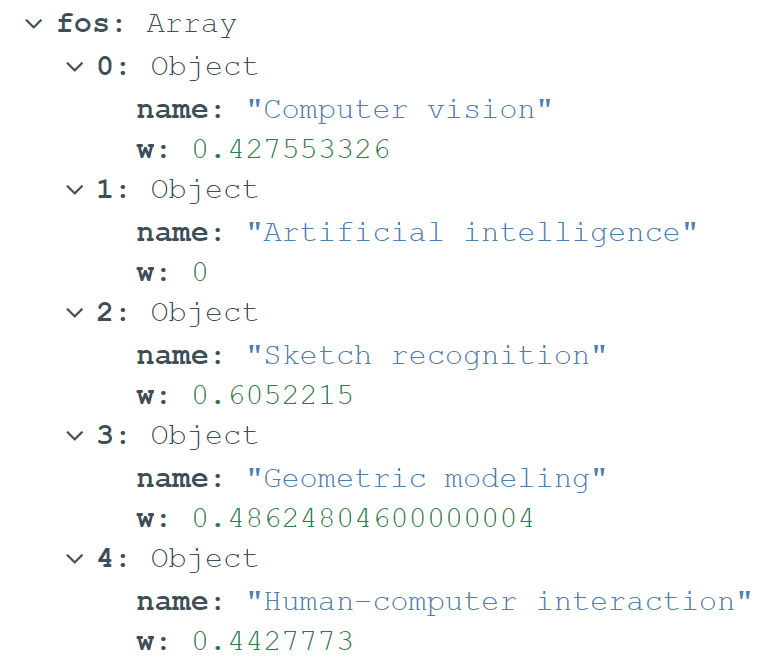
\includegraphics[width=0.6\textwidth]{Images/data/doc_fos.png}
    \caption{Structure of the \textit{fos} field}
\end{figure}

The \textit{references} field is implemented just as an array of ObjectIds.
 \begin{figure}[H]
    \centering
    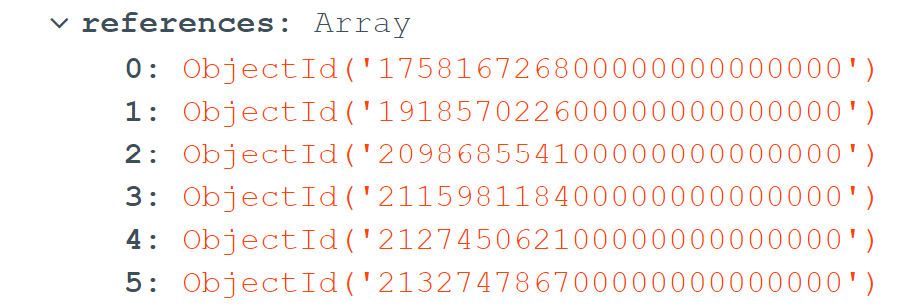
\includegraphics[width=0.7\textwidth]{Images/data/mongodb/doc_references.png}
    \caption{Structure of the \textit{references} field}
\end{figure}

\pagebreak
Lastly, the \textit{sections} field is an array of sub-documents. Each element of such array corresponds to one section of the paper. Every section can contain another array of sub-documents in the \textit{subsections} field and another array of sub-documents in the \textit{figures} field.
 \begin{figure}[H]
    \centering
    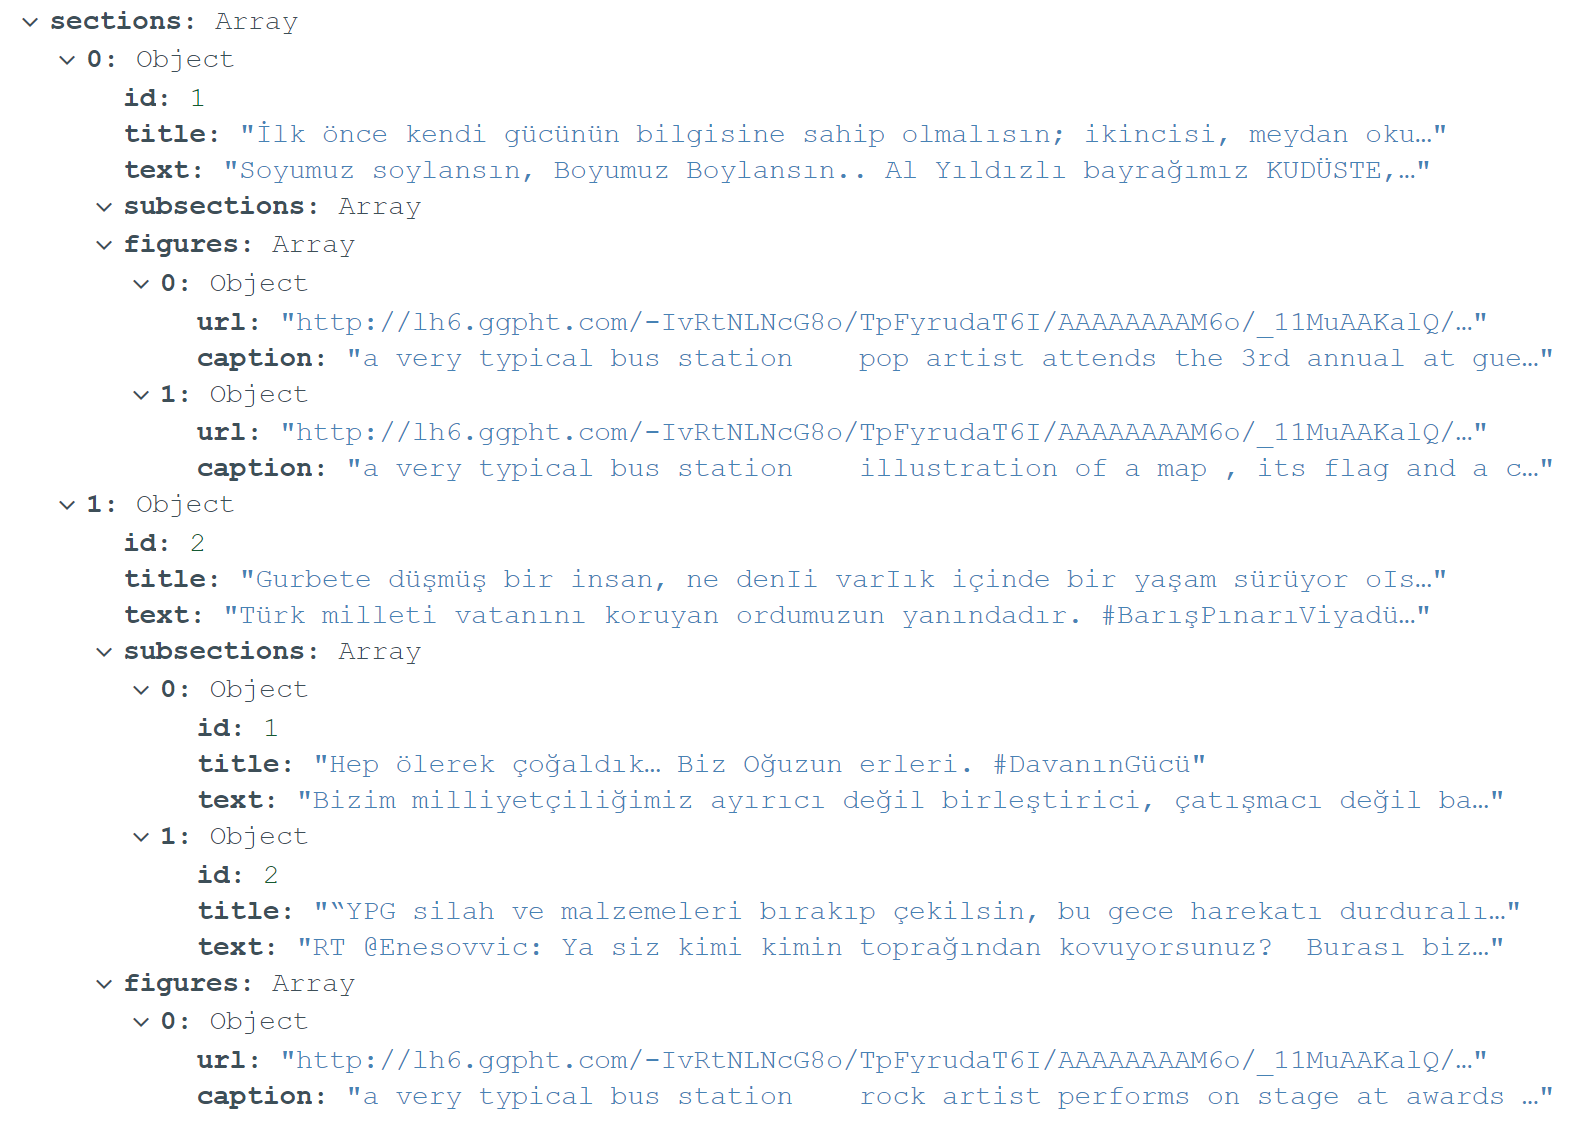
\includegraphics[width=\textwidth]{Images/data/doc_sections.png}
    \caption{Structure of the \textit{sections} field}
\end{figure}

\pagebreak
\subsection{Join Operation}
To get a temporary collection in which every document also contains an array with inside all the other documents it references, we can use the \textit{\$lookup} operator.
\inputminted[linenos,tabsize=2,breaklines]{MQL}{code/json/join.txt}
The referenced documents will be contained in the \textit{refs} field.

\subsection{Queries}
In this section queries with a different level of complexity are presented, with a brief description and a figure that shows their results. Notice that, for some queries, that return several documents, the result is only partially shown.
\begin{enumerate}

    \item \textbf{Find papers of 2006 with issue equal to 3 and volume greater or equal to 5. Then show just the list of authors with their name and organization, and also the venue of the paper. Limit the result to 2}:
    \inputminted[linenos,tabsize=2,breaklines]{MQL}{code/queries_mongodb/query_1.txt}
    (nReturned: 2, executionTimeMillis: 57, totalDocsExamined: 382)
    \begin{figure}[H]
        \centering
        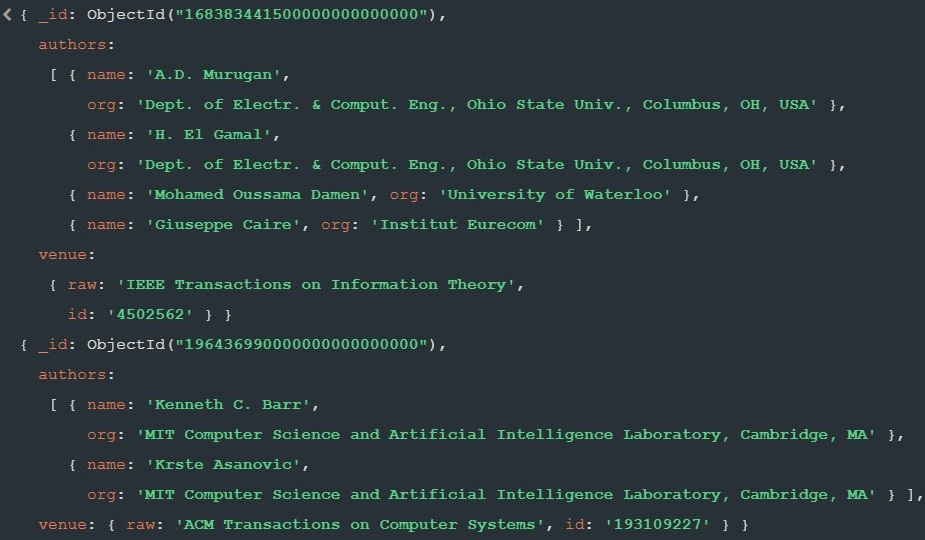
\includegraphics[width=0.8\textwidth]{Images/queries_mongodb/query_1.jpg}
    \end{figure}
    
    \item \textbf{Find 3 papers that were cited more than 500 times, published since 2015 in a Journal. Of them we retrieve only: title,
    publication year, number of citations, publisher, and doi}:
    \inputminted[linenos,tabsize=2,breaklines]{MQL}{code/queries_mongodb/query_2.txt}
    (nReturned: 3, executionTimeMillis: 3, totalDocsExamined: 326)
    \begin{figure}[H]
        \centering
        
\includegraphics[width=0.8\textwidth]{Images/queries_mongodb/query_2.jpg}
    \end{figure}

    \item \textbf{Find 5 papers that contain the word "artificial" in their abstract.\\
    To perform this query an index of type \textit{text}, on the field \textit{abstract} was previously created.}
    \inputminted[linenos,tabsize=2,breaklines]{MQL}{code/queries_mongodb/query_3.txt}
    (nReturned: 5, executionTimeMillis: 9, totalDocsExamined: 5)
    \begin{figure}[H]
        \centering
        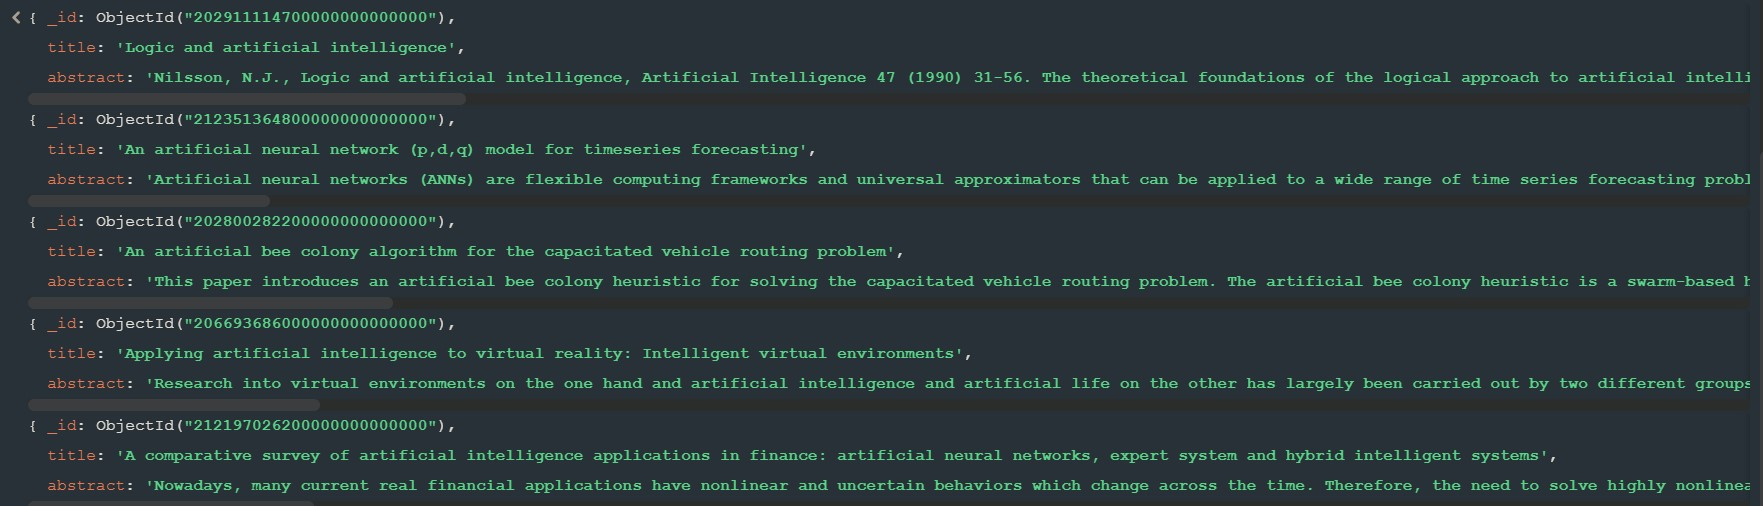
\includegraphics[width=0.9\textwidth]{Images/queries_mongodb/query_3.jpg}
    \end{figure}
    
    \item \textbf{Retrieve the sorted average number of pages, per doc\_type, of papers from a year after 2000, or with a number of citation greater or equal to 100}:
    \inputminted[linenos,tabsize=2,breaklines]{MQL}{code/queries_mongodb/query_4.txt}
    (nReturned: 3, executionTimeMillis: 195, totalDocsExamined: 8333)
    \begin{figure}[H]
        \centering
        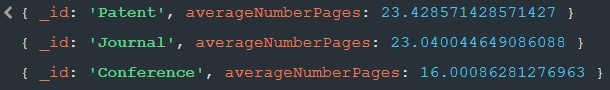
\includegraphics[width=0.8\textwidth]{Images/queries_mongodb/query_4.jpg}
    \end{figure}
    
    \item \textbf{Find the 7 papers that contain the most references, among the papers that cover a very relevant field of study (weight >= 0.7), and that were presented in a Conference}:
    \inputminted[linenos,tabsize=2,breaklines]{MQL}{code/queries_mongodb/query_5.txt}
    (nReturned: 7, executionTimeMillis: 14, totalDocsExamined: 8333)
    \begin{figure}[H]
        \centering
        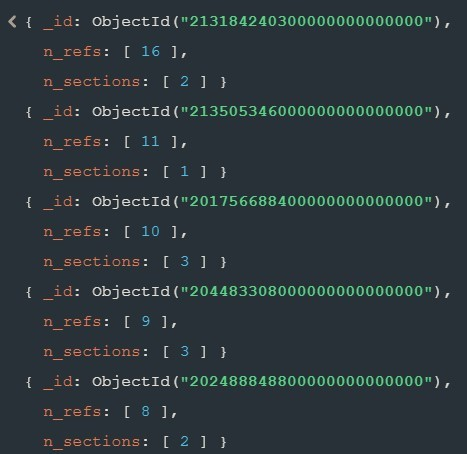
\includegraphics[width=0.7\textwidth]{Images/queries_mongodb/query_5_1.jpg}
        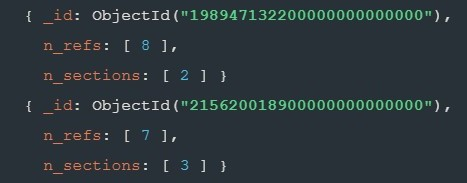
\includegraphics[width=0.7\textwidth]{Images/queries_mongodb/query_5_2.jpg}
    \end{figure}
    
    \item \textbf{Find the papers whose fos (field of studies) is "Computer engineering" or "Computer science", and that have at least one subsection}:
    \inputminted[linenos,tabsize=2,breaklines]{MQL}{code/queries_mongodb/query_6.txt}
    (nReturned: 1789, executionTimeMillis: 31, totalDocsExamined: 8333)
    \begin{figure}[H]
        \centering
        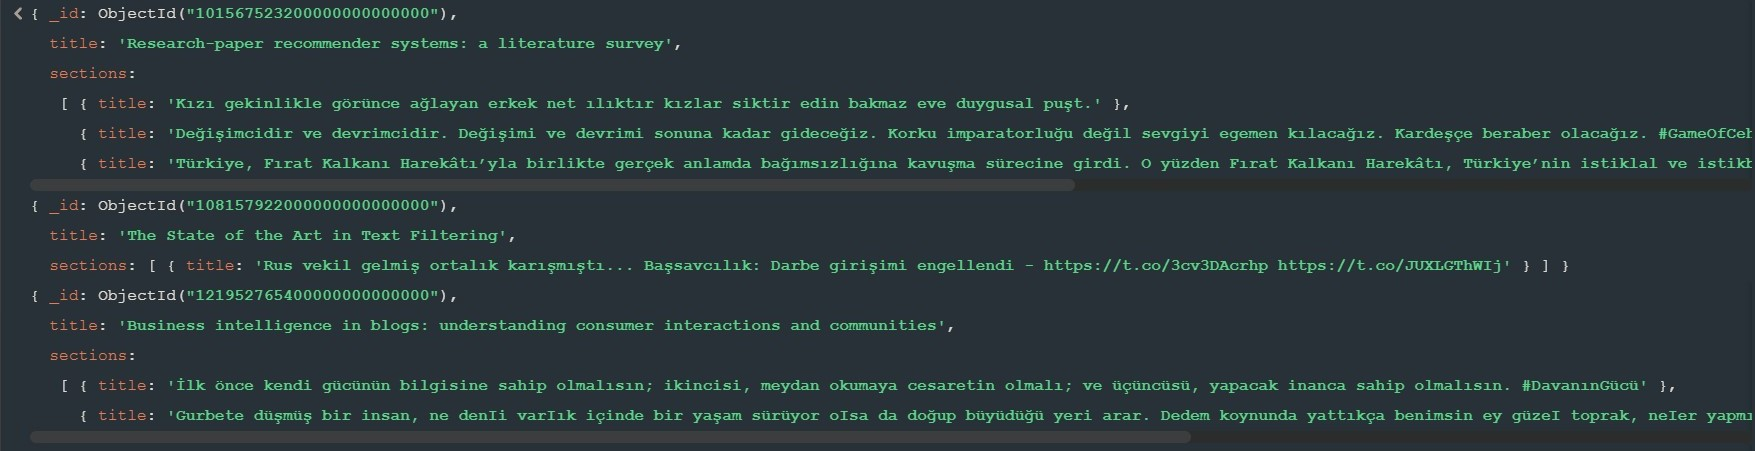
\includegraphics[width=0.9\textwidth]{Images/queries_mongodb/query_6.jpg}
    \end{figure}
    
    \item \textbf{Find 10 papers with author affiliated with "IEEE", that have 3 sections and at least a figure's caption containing the word "bus"}:
    \inputminted[linenos,tabsize=2,breaklines]{MQL}{code/queries_mongodb/query_7.txt}
    (nReturned: 10, executionTimeMillis: 21, totalDocsExamined: 7247)
    \begin{figure}[H]
        \centering
        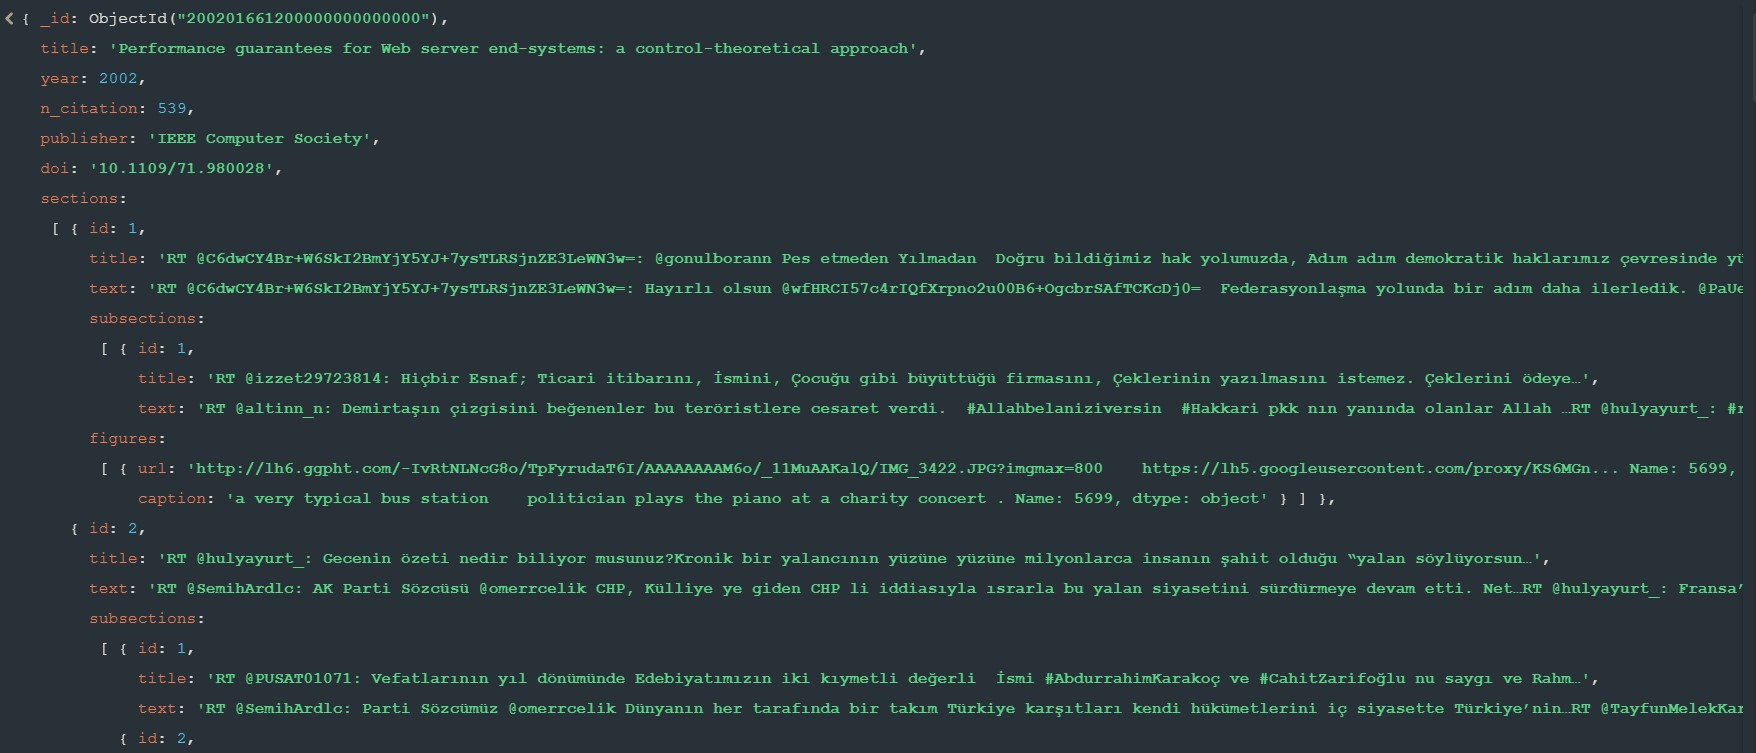
\includegraphics[width=0.8\textwidth]{Images/queries_mongodb/query_7_1.jpg}
        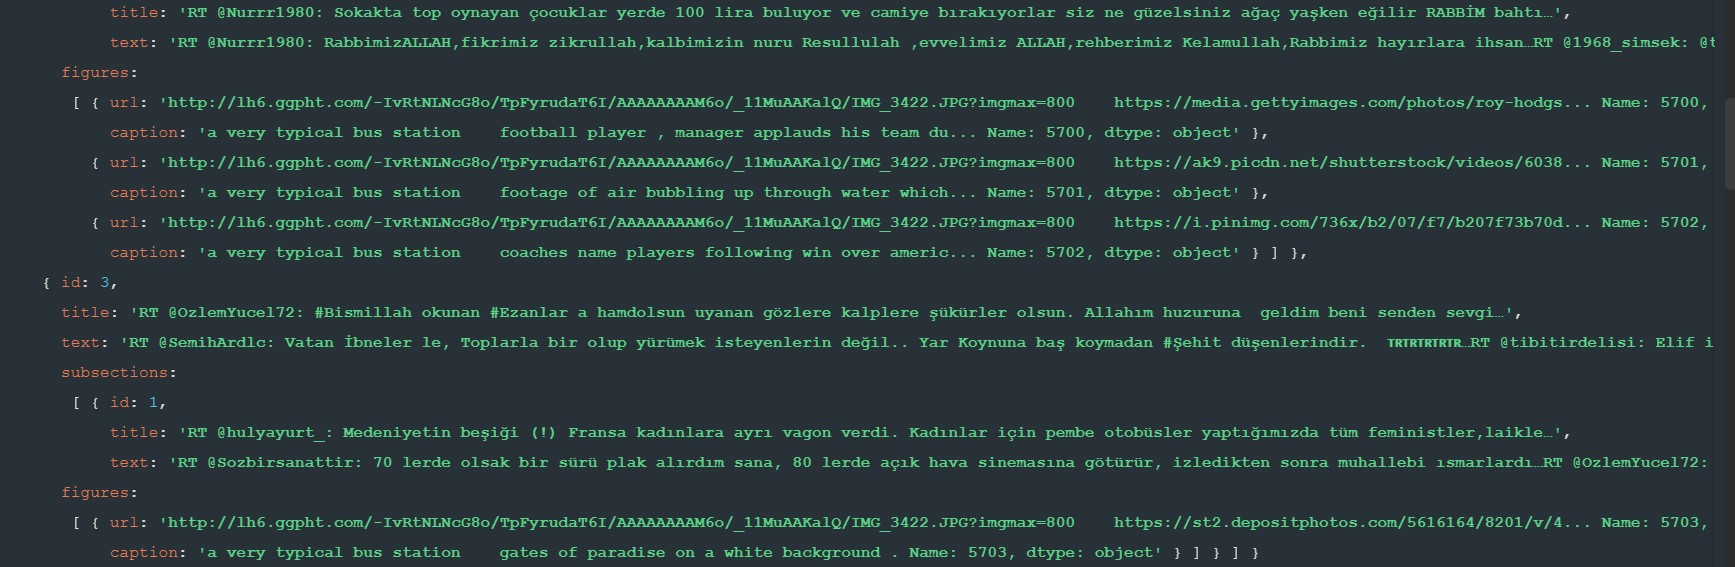
\includegraphics[width=0.8\textwidth]{Images/queries_mongodb/query_7_2.jpg}
    \end{figure}
    
    \pagebreak
    \item \textbf{Retrieve for each venue the content of the papers, with more than 500 citations, and volume greater than 12, published in it.}
    
    \textbf{This is done by first matching the conditions stated above, then unwinding on the sub-document "sections". In the end grouping by venue, and retrieving the sections, we obtain the following results (for each venue, an array with the contents collected from all the papers published in it)}:
    \inputminted[linenos,tabsize=2,breaklines]{MQL}{code/queries_mongodb/query_8.txt}
    (nReturned: 923, executionTimeMillis: 126, totalDocsExamined: 8333)
    \begin{figure}[H]
        \centering
        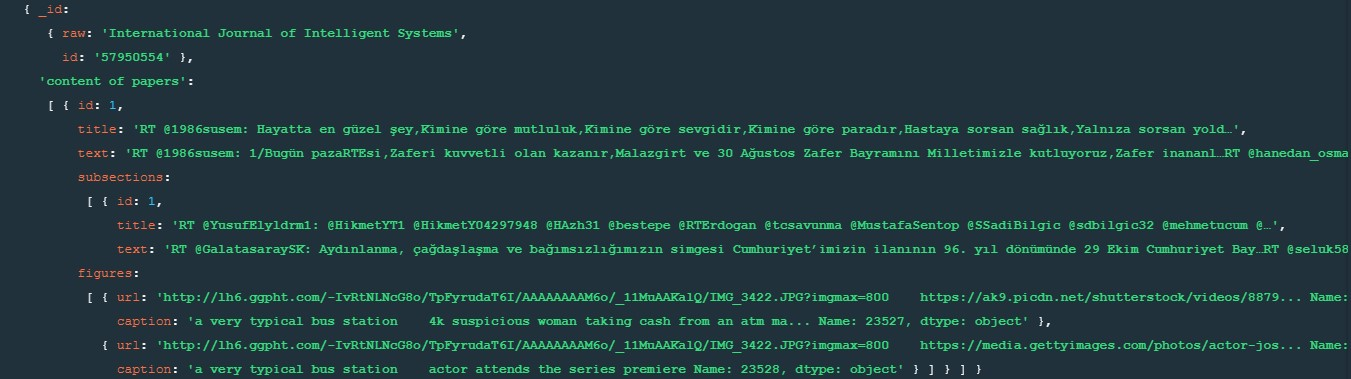
\includegraphics[width=0.8\textwidth]{Images/queries_mongodb/query_8_1.jpg}
        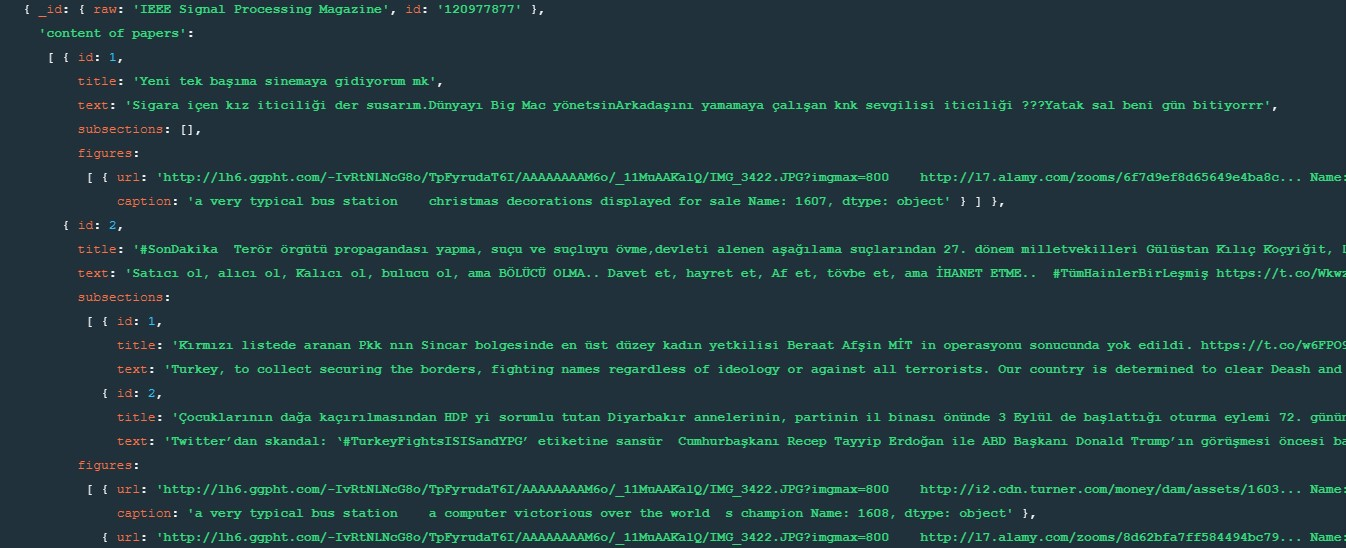
\includegraphics[width=0.8\textwidth]{Images/queries_mongodb/query_8_2.jpg}
        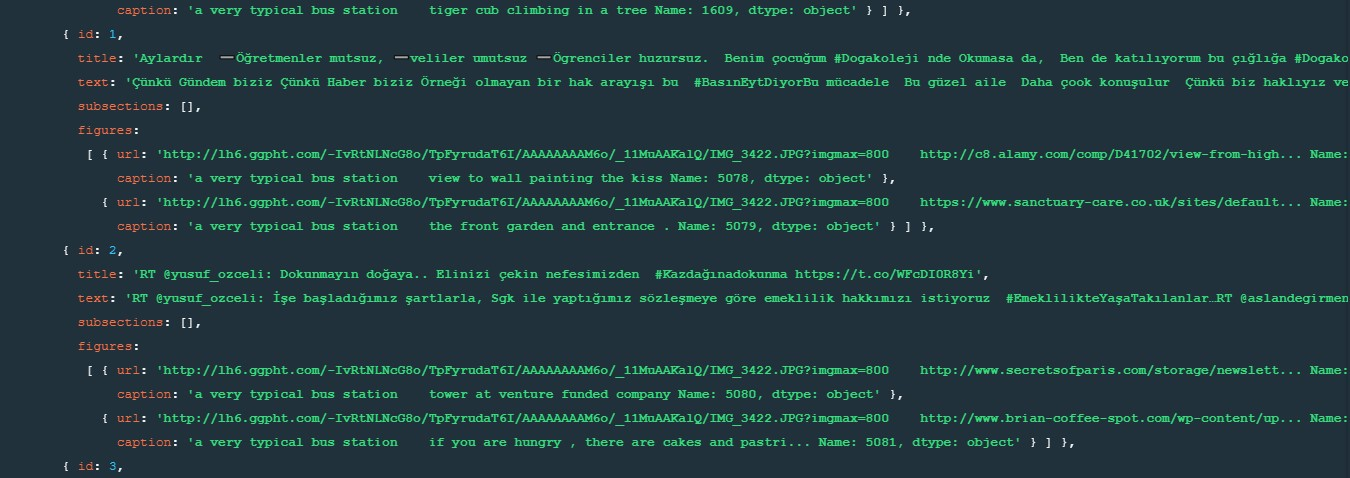
\includegraphics[width=0.8\textwidth]{Images/queries_mongodb/query_8_3.jpg}
    \end{figure}
    
    \pagebreak
    \item \textbf{Find the number of papers of the first 10 authors, affiliated to an University, that wrote most papers in Journals after year 2000.}
    
    \textbf{This is done by first matching the conditions, and unwinding on the sub-documents "authors". Then by grouping by \textit{authors.id}, the number of papers for each author can be computed. In the end the results are sorted, and the first 10 are shown.}
    \inputminted[linenos,tabsize=2,breaklines]{MQL}{code/queries_mongodb/query_9.txt}
    (nReturned: 10, executionTimeMillis: 256, totalDocsExamined: 8333)
    \begin{figure}[H]
        \centering
        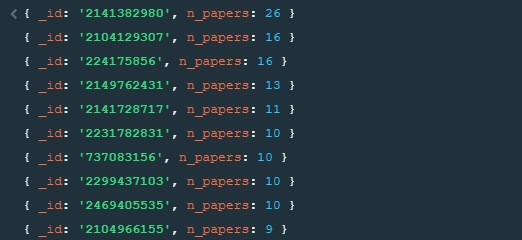
\includegraphics[width=0.6\textwidth]{Images/queries_mongodb/query_9.jpg}
    \end{figure}
    
    \item \textbf{Find the referenced papers whose \textit{fos} (field of studies) is "Data mining" and whose volume is 3, and that have at least one section}:
    \inputminted[linenos,tabsize=2,breaklines]{MQL}{code/queries_mongodb/query_10.txt}
    (nReturned: 24, executionTimeMillis: 37, totalDocsExamined: 8333)
    \begin{figure}[H]
        \centering
        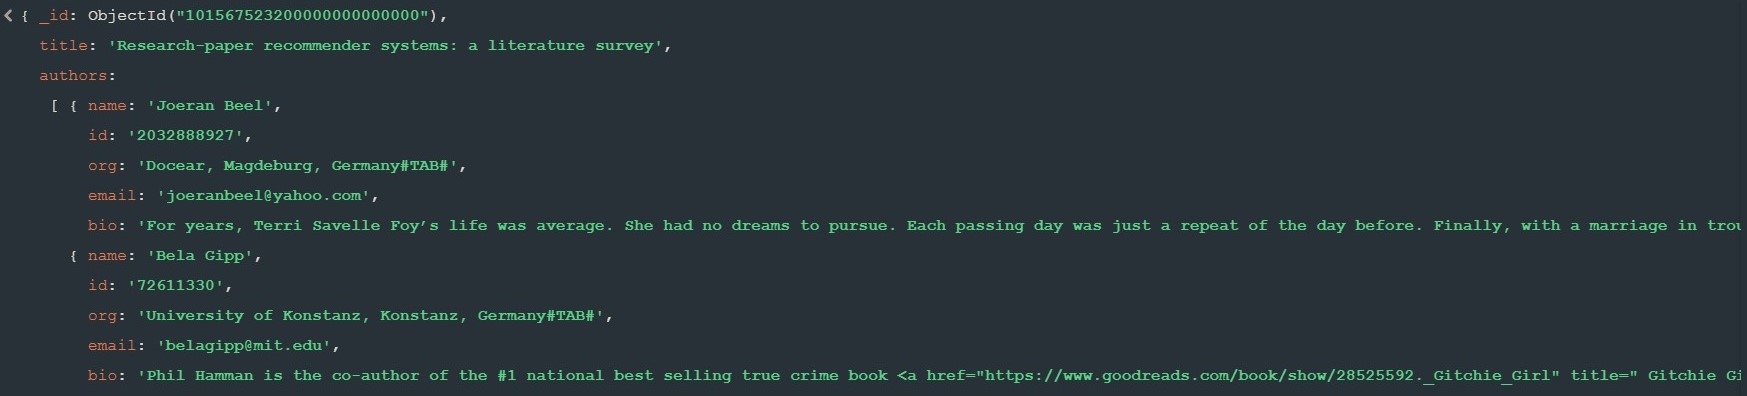
\includegraphics[width=0.8\textwidth]{Images/queries_mongodb/query_10_1.jpg}
         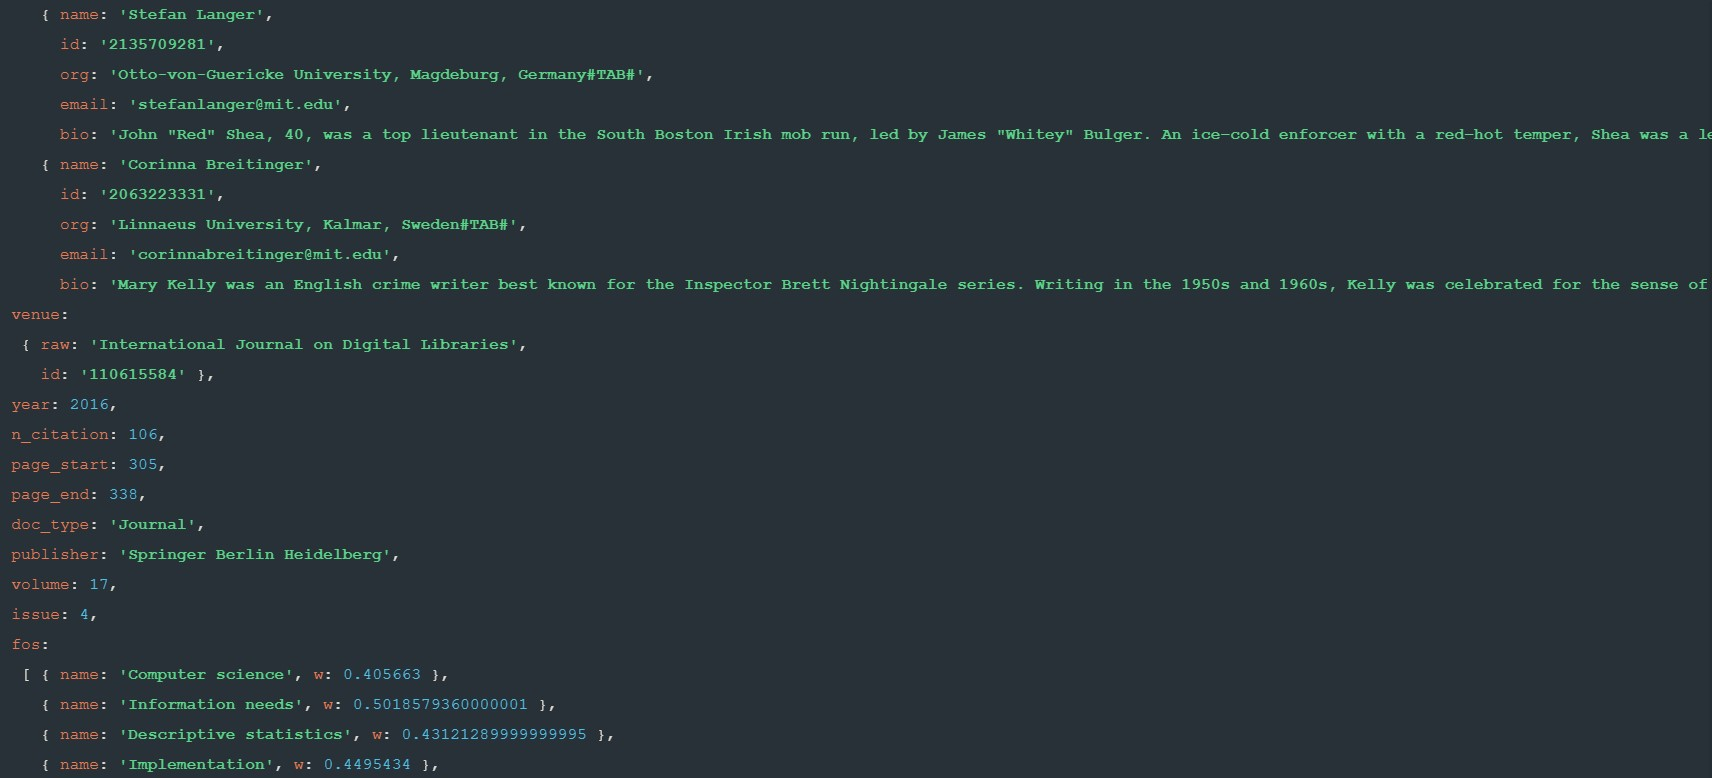
\includegraphics[width=0.8\textwidth]{Images/queries_mongodb/query_10_2.jpg}        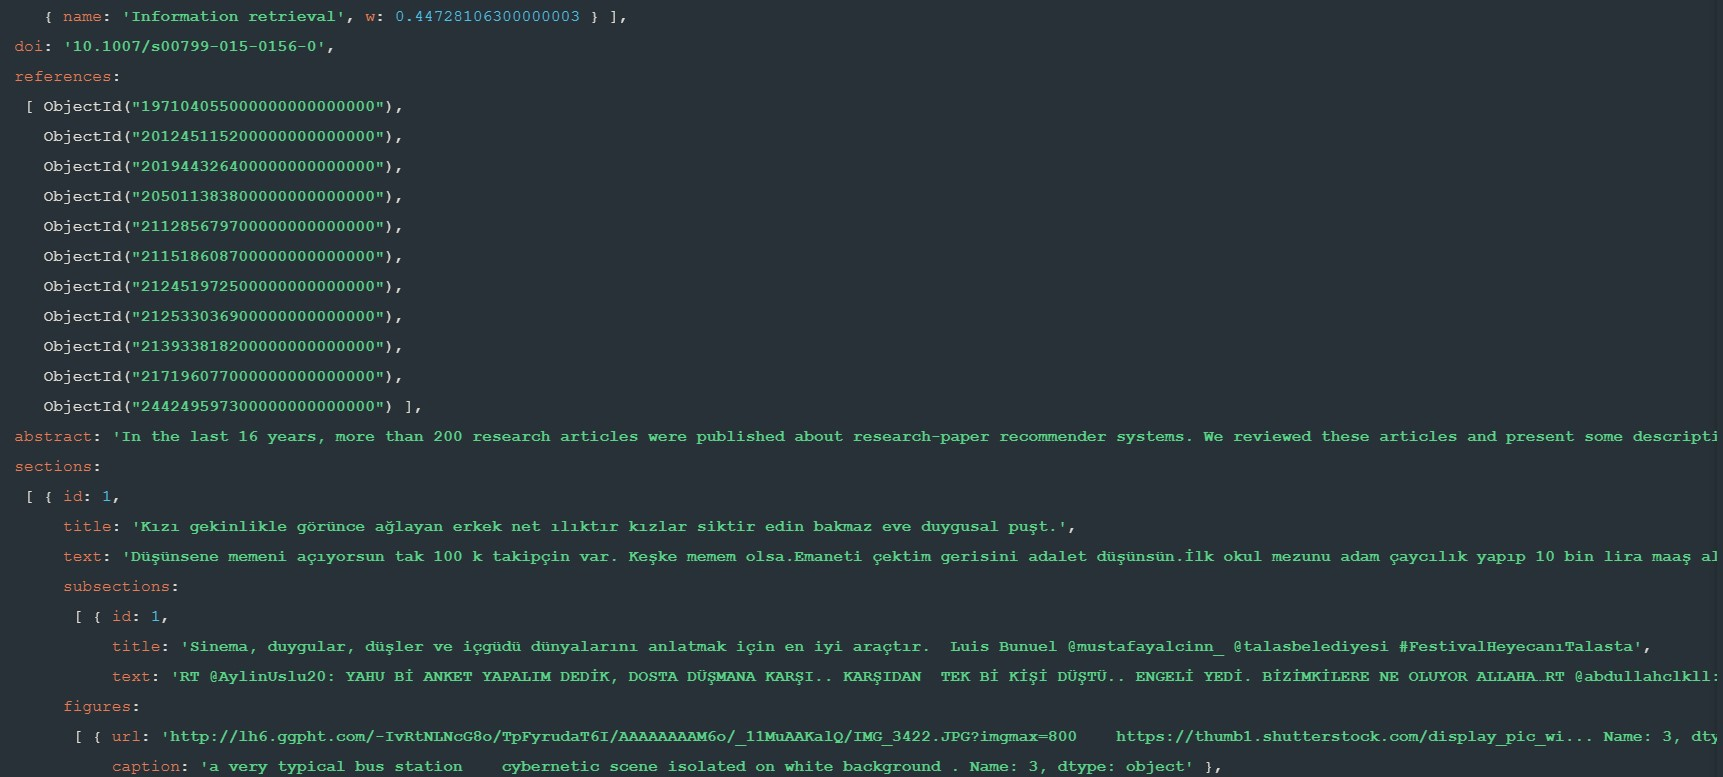
\includegraphics[width=0.8\textwidth]{Images/queries_mongodb/query_10_3.jpg}
     \end{figure}
     \begin{figure}[H]
        \centering
        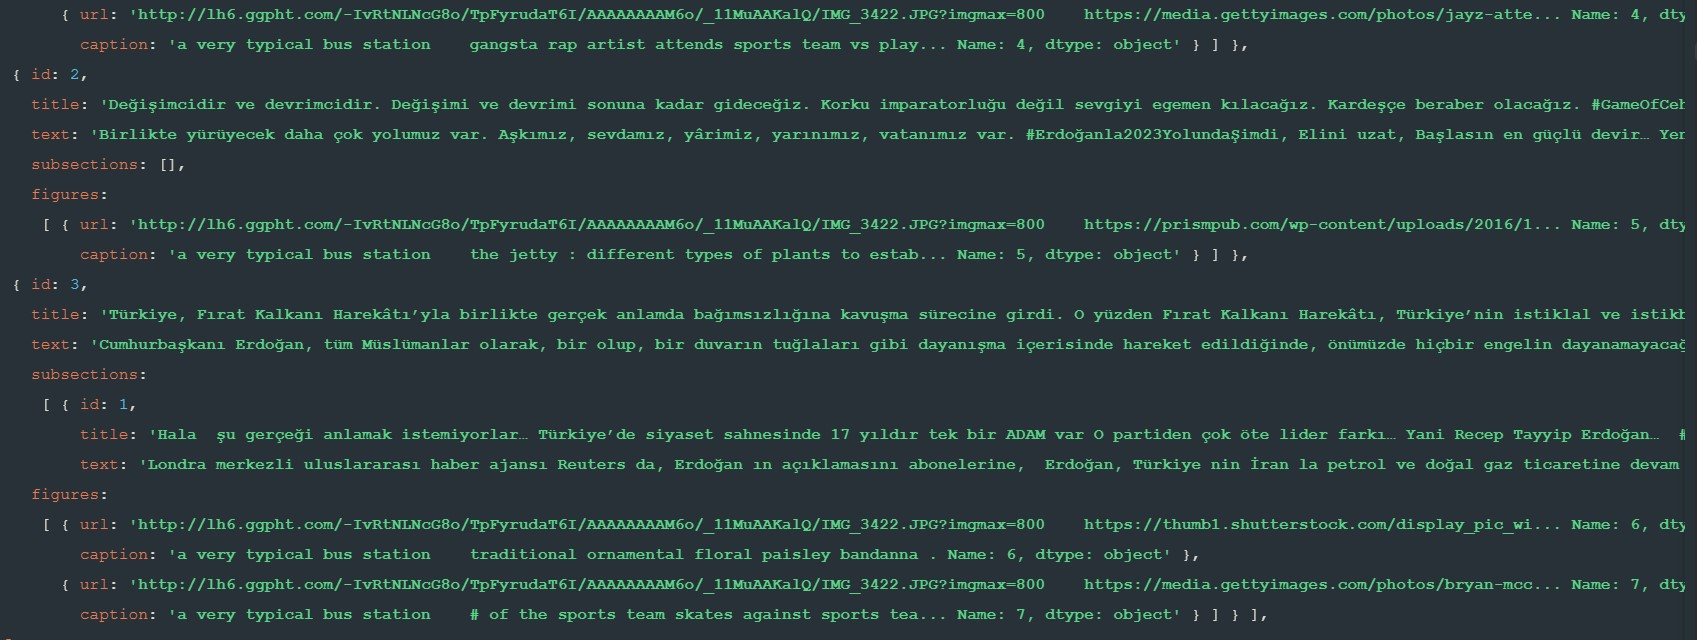
\includegraphics[width=0.8\textwidth]{Images/queries_mongodb/query_10_4.jpg}
        \includegraphics[width=0.8\textwidth]{Images/queries_mongodb/query_10_5.jpg}
    \end{figure}
    
    \item \textbf{Find papers that are referenced by papers regarding machine learning, written by an IEEE author or published by "IEEE Computer Society" after 2010. Of the referenced papers retrieved with the join, show id, title and year of the ones published before 2005}:
    \inputminted[linenos,tabsize=2,breaklines]{MQL}{code/queries_mongodb/query_11.txt}
    (nReturned: 8, executionTimeMillis: 79, totalDocsExamined: 8333)
    \begin{figure}[H]
        \centering
        \includegraphics[width=0.8\textwidth]{Images/queries_mongodb/query_11_1.jpg}
        \includegraphics[width=0.8\textwidth]{Images/queries_mongodb/query_11_2.jpg}
        \includegraphics[width=0.8\textwidth]{Images/queries_mongodb/query_11_3.jpg}
    \end{figure}
    \begin{figure}[H]
        \centering
        \includegraphics[width=0.8\textwidth]{Images/queries_mongodb/query_11_4.jpg}
        \includegraphics[width=0.8\textwidth]{Images/queries_mongodb/query_11_5.jpg}
    \end{figure}
    
\end{enumerate}

\subsection{Creation/Update Commands}
\begin{enumerate}
    \item \textbf{Deletion of one paper from the database}:
    \inputminted[linenos,tabsize=2,breaklines]{MQL}{code/commands_mongodb/cmd_1.txt}
    \item \textbf{Deletion of some papers, based on some conditions}:
    \inputminted[linenos,tabsize=2,breaklines]{MQL}{code/commands_mongodb/cmd_2.txt}
    \item \textbf{Insertion of a new paper}:
    \inputminted[linenos,tabsize=2,breaklines]{MQL}{code/commands_mongodb/cmd_3.txt}
    \item \textbf{Insertion of more papers at once}:
    \inputminted[linenos,tabsize=2,breaklines]{MQL}{code/commands_mongodb/cmd_4.txt}
    \item \textbf{Update of a paper, by modification of the title of a subsection}:
    \inputminted[linenos,tabsize=2,breaklines]{MQL}{code/commands_mongodb/cmd_5.txt}
    \item \textbf{Update some papers, based on some conditions, modifying starting and ending pages}:
    \inputminted[linenos,tabsize=2,breaklines]{MQL}{code/commands_mongodb/cmd_6.txt}
\end{enumerate}


\chapter{References}
\label{ch:references}
\begin{itemize}
    \item \textbf{\href{https://www.aminer.org/citation}{Aminer data set}}
    \item \textbf{\href{https://www.kaggle.com/datasets/choobani/goodread-authors}{Bio data set}}
    \item \textbf{\href{https://transparency.twitter.com/en/reports/moderation-research.html}{Tweets data set}}
    \item \textbf{\href{https://huggingface.co/datasets/conceptual_captions/commit/0477f735cc48e10c43ef55b9b2ca67fce3d45314\#d2h-548657}{Images data set}}
    \item \textbf{\href{https://app.diagrams.net/}{Draw.io}}
    \item \textbf{\href{https://neo4j.com/}{Neo4j}}
    \item \textbf{\href{https://www.mongodb.com/}{MongoDB}}
    \item \textbf{\href{https://www.overleaf.com/}{Overleaf}}
    \item \textbf{\href{https://www.python.org/}{Python}}
\end{itemize}
\end{document}